% compile with XeLaTeX
\documentclass[dvipsnames,mathserif]{beamer}



\def\norm#1{\left\|#1\right\|}

\newcommand{\D}{D}
\newcommand{\Lun}{L}
\newcommand{\Lsym}{L_{\text{sym}}}
\newcommand{\Lrw}{L_{\text{rw}}}
\renewcommand{\bar}{\overline} %

\DeclareMathOperator{\Tr}{Tr}%
\DeclareMathOperator{\vol}{vol} %
\DeclareMathOperator{\Ratiocut}{RatioCut}
\DeclareMathOperator{\Ncut}{Ncut}
\DeclareMathOperator{\Cut}{cut}
\DeclareMathOperator{\Mincut}{MinCut}
\DeclareMathOperator{\MinmaxCut}{MinMaxCut}

 

%\usepackage{xcolor}% http://ctan.org/pkg/xcolor
%\usepackage{colortbl}% http://ctan.org/pkg/colortbl
%%\def\pedro#1{\textcolor{magenta}{#1}} 
%\usepackage[utf8]{inputenc}
%\usepackage{amsfonts}
%%%%%%%%%%%%%%%%%%%%%%%%%%%%%%%%%%%%%%%%%%%
%%%%%%%%%%%%%%%%%%%%%%%%%%%%%%%%%%%%%%%%%%%
%%%%%%%%%%%%%%%%%%%%%%%%%%%%%%%%%%%%%%%%%%%
%   
%\pagestyle{plain}
%\usepackage[numbers]{natbib}
% Comment this out before submission to drop the page numbers 

%%%%
%%%%
%%%  From Dropbox
%%%


\newcommand\x{\times}
\newcommand\bigzero{\makebox(0,0){\text{\huge0}}}
\newcommand*{\bord}{\multicolumn{1}{c|}{}}
 
\newcommand{\Ln}{L^{-}}
\newcommand{\Lp}{L^{+}}
\newcommand{\Dn}{D^{-}}
\newcommand{\Dp}{D^{+}}
 
\newcommand{\Tbar }{ \bar{T} }
 
\newcommand{\ELn }{   \expec{[\Ln]}  }
\newcommand{\ELp }{   \expec{[\Lp]}  }

\newcommand{\EDp }{   \expec{[\Dp]}  }
\newcommand{\EDn }{   \expec{[\Dn]}  }

    
\newcommand{\An}{A^{-}}
\newcommand{\Ap}{A^{+}}
\newcommand{\EAp }{   \expec{[\Ap]}  }
\newcommand{\EAn }{   \expec{[\An]}  }



\usepackage{tikz}
\usetikzlibrary{matrix,decorations.pathreplacing,calc}

% Set various styles for the matrices and braces. It might pay off to fiddle around with the values a little bit
\pgfkeys{tikz/mymatrixenv/.style={decoration=brace,every left delimiter/.style={xshift=3pt},every right delimiter/.style={xshift=-3pt}}}
\pgfkeys{tikz/mymatrix/.style={matrix of math nodes,left delimiter=[,right delimiter={]},inner sep=2pt,column sep=1em,row sep=0.5em,nodes={inner sep=0pt}}}
\pgfkeys{tikz/mymatrixbrace/.style={decorate,thick}}
\newcommand\mymatrixbraceoffseth{0.5em}
\newcommand\mymatrixbraceoffsetv{0.2em}

% Now the commands to produce the braces. (I'll explain below how to use them.)
\newcommand*\mymatrixbraceright[4][m]{
    \draw[mymatrixbrace] ($(#1.north west)!(#1-#3-1.south west)!(#1.south west)-(\mymatrixbraceoffseth,0)$)
        -- node[left=2pt] {#4} 
        ($(#1.north west)!(#1-#2-1.north west)!(#1.south west)-(\mymatrixbraceoffseth,0)$);
}
\newcommand*\mymatrixbraceleft[4][m]{
    \draw[mymatrixbrace] ($(#1.north east)!(#1-#2-1.north east)!(#1.south east)+(\mymatrixbraceoffseth,0)$)
        -- node[right=2pt] {#4} 
        ($(#1.north east)!(#1-#3-1.south east)!(#1.south east)+(\mymatrixbraceoffseth,0)$);
}
\newcommand*\mymatrixbracetop[4][m]{
    \draw[mymatrixbrace] ($(#1.north west)!(#1-1-#2.north west)!(#1.north east)+(0,\mymatrixbraceoffsetv)$)
        -- node[above=2pt] {#4} 
        ($(#1.north west)!(#1-1-#3.north east)!(#1.north east)+(0,\mymatrixbraceoffsetv)$);
}
\newcommand*\mymatrixbracebottom[4][m]{
    \draw[mymatrixbrace] ($(#1.south west)!(#1-1-#3.south east)!(#1.south east)-(0,\mymatrixbraceoffsetv)$)
        -- node[below=2pt] {#4} 
        ($(#1.south west)!(#1-1-#2.south west)!(#1.south east)-(0,\mymatrixbraceoffsetv)$);
}

  
\newcommand{\mydef}{\stackrel{\text{def}}{=}}
\newcommand{\mydeff}{ \coloneqq }
 
\newcommand{\omo}{ \mb{1}_{C, \bar{C}}  }

% \usepackage{nicematrix}
% \NiceMatrixOptions{transparent,nullify-dots}
 
\newcommand{\tce}{   \tilde{c}_{\varepsilon}  }

%-----------------------------------------
% Some commands defined by Hemant
%----------------------------------------- 
\newcommand{\EA }{   \expec{[A]}  }
% ????  \newcommand{\Dbar }{ \bar{D} } 
\newcommand{\EDbar }{   \expec{[\Dbar]}  }
\newcommand{\Dbarn }{ \bar{D}^{-} }
\newcommand{\Dbarp }{ \bar{D}^{+} }
\newcommand{\Lbar }{ \bar{L} }
\newcommand{\ELbar }{   \expec{[\Lbar]}  }

% \newcommand{\mb}[1]{\mbox{\boldmath$#1$}}
\newcommand{\ones }{ \mb{1} }

\newcommand{\infovec }{w}
\newcommand{\pert }{\tri}

\newcommand{\Gn }{ G^{-} }
\newcommand{\Gp }{ G^{+} }

\newcommand{\taup }{ \tau^{+} }
\newcommand{\taun }{ \tau^{-} }



% Miscellaneous symbols 
\newcommand{\tri}{\ensuremath{\bigtriangleup}}

\newcommand{\ceil}[1]{\lceil{#1}\rceil}
\newcommand{\floor}[1]{\lfloor{#1}\rfloor}
\newcommand{\set}[1]{\left\{{#1}\right\}}
\newcommand{\dotprod}[2]{\langle#1,#2\rangle}
\newcommand{\est}[1]{\widehat{#1}}
\newcommand{\expec}{\ensuremath{\mathbb{E}}}
\newcommand{\grad}{\ensuremath{\nabla}}
\newcommand{\hess}{\ensuremath{\nabla^2}}
\newcommand{\matR}{\ensuremath{\mathbb{R}}}
\newcommand{\matZ}{\ensuremath{\mathbb{Z}}}
\newcommand{\argmax}[1]{\underset{#1}{\operatorname{argmax}}}
\newcommand{\argmin}[1]{\underset{#1}{\operatorname{argmin}}}
\newcommand{\ubar}[1]{\underaccent{\bar}{#1}}
\newcommand{\prob}{\ensuremath{\mathbb{P}}}
\newcommand{\Linfnorm}{L_{\infty}}
\newcommand{\vp}{\ensuremath{v^{\prime}}}
\newcommand{\vpp}{\ensuremath{v^{\prime\prime}}}
\newcommand{\tp}{\ensuremath{t^{\prime}}}
\newcommand{\lp}{\ensuremath{l^{\prime}}}
\newcommand{\qp}{\ensuremath{q^{\prime}}}


\newcommand{\red}[1]{\textcolor{red}{#1}}
\newcommand{\blue}[1]{\textcolor{blue}{#1}}


\setbeamersize{text margin left=12pt,text margin right=12pt}


\setbeamertemplate{footline}[frame number]
\setbeamercolor{footline}{fg=black}
\setbeamerfont{footline}{series=\bfseries}
\setbeamerfont{footnote}{size=\tiny}
\usepackage{tikz}
\usepackage{caption}
\captionsetup{font=scriptsize,labelfont=scriptsize}
\usepackage[backend=biber,style=authoryear]{biblatex}
\addbibresource{sample-base.bib}

% \DeclareMathOperator*{\argmax}{argmax}
%\usetheme{Frankfurt}%1
\usetheme{Darmstadt}%1

% for RTL liste
\makeatletter
\newcommand{\RTListe}{\raggedleft\rightskip\leftm}
\newcommand{\leftm}{\@totalleftmargin}
\makeatother

% RTL frame title
\setbeamertemplate{frametitle}
{\vspace*{-1mm}
  \nointerlineskip
    \begin{beamercolorbox}[sep=0.3cm,ht=1.8em,wd=\paperwidth]{frametitle}
        \vbox{}\vskip-2ex%
        \strut\hskip1ex\insertframetitle\strut
        \vskip-0.8ex%
    \end{beamercolorbox}
}
% align subsection in toc
\makeatletter
\setbeamertemplate{subsection in toc}
{\leavevmode\rightskip=5ex%
  \llap{\raise0.1ex\beamer@usesphere{subsection number projected}{bigsphere}\kern1ex}%
  \inserttocsubsection\par%
}
\makeatother

% RTL triangle for itemize
\setbeamertemplate{itemize item}{\scriptsize\raise1.25pt\hbox{\donotcoloroutermaths$\blacktriangleright$}} 

%\setbeamertemplate{itemize item}{\rule{4pt}{4pt}}

\defbeamertemplate{enumerate item}{square2}
{\LR{
    %
    \hbox{%
    \usebeamerfont*{item projected}%
    \usebeamercolor[bg]{item projected}%
    \vrule width2.25ex height1.85ex depth.4ex%
    \hskip-2.25ex%
    \hbox to2.25ex{%
      \hfil%
      {\color{fg}\insertenumlabel}%
      \hfil}%
  }%
}}

\setbeamertemplate{enumerate item}[square2]
\setbeamertemplate{navigation symbols}{}

\usepackage{ifthen}

\newboolean{withPause}
\newboolean{withPause2}

\newcommand\myp{\ifthenelse{\boolean{withPause}}{ \pause }{}}

\newcommand\mypv{\vfill \ifthenelse{\boolean{withPause}}{ \pause }{}}


\setboolean{withPause}{true}
% \setboolean{withPause}{false}





\usepackage{color}

\newcommand*{\bluebullet}{\textcolor{blue}{\textbullet} }
\newcommand{\bb}{\bluebullet}

 
% \titlegraphic { 
% \begin{tikzpicture}[overlay,remember picture, opacity=0.1,]
% \node[] at (0, 2.9){
%     \includegraphics[width=0.63\textwidth]{Logo_uzad.pdf}
% };\end{tikzpicture}}
\setbeamertemplate{caption}[numbered]
\begin{document}

\rightskip\rightmargin
\title{Cluster-driven Hierarchical Representation of Large Asset Universes for Optimal Portfolio Construction}
% \author{ \large Mihai Cucuringu}

% \institute{Department of Statistics \& Mathematical Institute\\   Oxford-Man Institute of Quantitative Finance\\   University of Oxford\\   The Alan Turing Institute}

% \footnotesize{\date{\today }
% \footnotesize{\date{ November 16, 2024}

\begin{frame}
\maketitle
\begin{center}
\footnotesize
   %  {Nail Khelifa, Jerome Allier (ENSAE), }
    Nail Khelifa, Jérôme Allier, and Mihai Cucuringu. \\
    In Proceedings of the 5th ACM International Conference on AI in Finance (ICAIF '24). Association for Computing Machinery, New York, NY, USA, 177–185
\end{center}
\end{frame}

\begin{frame}{Summary}
\footnotesize \tableofcontents
\end{frame}





\section{Introduction}
%%%%%%%%%%%%%%%%%%%%%%%%%%%%%%%%%%%%%%%%%%%%%%%%%%%%%%%%%%%%
\begin{frame}{\large Problem setup \& methodology overview}
\vfill
\footnotesize 
    \vspace{-1mm}  
    \textbf{Motivation}:
    \begin{itemize}
        \item Traditional Markowitz portfolio construction faces challenges in large asset universes: ill-conditioned covariance \&  curse of dimensionality.
    \end{itemize}
\mypv     
    \textbf{Our Approach:}
    \begin{itemize}
        \item We propose a  \red{\textit{hierarchical framework}} that facilitates Markowitz optimization for large portfolios: clustering highly correlated assets to construct  \red{\textit{cluster indices} (synthetic ETFs)}, effectively reducing dimensionality
    \end{itemize}
\mypv     
    \textbf{Methodology}:
    \begin{itemize}
        \item Interpret the correlation matrix as a \red{signed graph}, where:
            \begin{itemize}
                \item nodes represent assets
                \item edges encode correlations between assets
            \end{itemize}            
        \mypv 
        \item Apply \red{\textit{signed spectral clustering}} to form asset clusters
        \item Assign Gaussian intra-cluster weights for the constituent assets (cluster indices)  
        \item Conduct Markowitz optimization on the resulting cluster indices 
        % to infer a weight for each cluster
        \item Map back to the original space to infer weights for individual assets  
    \end{itemize}
\mypv 
    \textbf{Results:}
    \begin{itemize}
        \item Demonstrate superior performance over traditional methods and benchmarks in terms of volatility and returns.
    \end{itemize}
\vfill
\end{frame}
%%%%%%%%%%%%%%%%%%%%%%%%%%%%%%%%%%%%%%%%%%%%%%%%%%%%%%%%%%%%




%%%%%%%%%%%%%%%%%%%%%%%%%%%%%%%%%%%%%%%%%%%%%%%%%%%%%%%%%%%%
\begin{frame}{Markowitz Portfolio Optimization}
\vfill
\begin{itemize}
    \item \textbf{Framework}: Markowitz Mean-Variance Optimization (\cite{MarkowitzPO}).
    \item \textbf{Objective}: find the lowest volatility portfolio achieving a target return $\rho_0$.
\end{itemize}


\bigskip 
    \begin{columns}
        \column{0.6\textwidth}

        \textbf{Optimization Problem:}
        
        \begin{equation*}
            (\boldsymbol{\mathcal{M}}) ~~
            \left\{
                \begin{array}{ll}
                    \underset{\boldsymbol{\omega}}{\min} ~ \boldsymbol{\omega}^T\boldsymbol{\Sigma}\boldsymbol{\omega} \\
                    \text{s.t. } \boldsymbol{\omega}^T \bar{r} \geq \rho_0, \\
                    \sum_{i=1}^n \omega_i = 1.
                \end{array}
            \right.
        \end{equation*}

        \column{0.4\textwidth}
        
        \textbf{Variables:}

        \bigskip
        \centering
        \begin{itemize}
            \item \( \boldsymbol{\omega} \): Portfolio weights
            \item \( \bar{r} \): Expected returns
            \item \( \boldsymbol{\Sigma} \): Covariance matrix
            \item \( \rho_0 \): Target return level
        \end{itemize}

    \end{columns}
\vfill
\end{frame}
%%%%%%%%%%%%%%%%%%%%%%%%%%%%%%%%%%%%%%%%%%%%%%%%%%%%%%%%%%%%



%%%%%%%%%%%%%%%%%%%%%%%%%%%%%%%%%%%%%%%%%%%%%%%%%%%%%%%%%%%%
\begin{frame}{Motivation: why clustering?}

\vfill 

\textbf{Key Issues}
\begin{enumerate}
    \item \textbf{Estimation of \( \boldsymbol{\Sigma} \):}
        \begin{itemize}
            \item When the number of assets \( n \) is large (\( n = 695 \) in our work), estimating the \( \frac{n(n+1)}{2} \) coefficients of \( \boldsymbol{\Sigma} \) becomes problematic with limited observations (a common issue in practice): the curse of dimensionality.
        \end{itemize}

    % \mypv   
    \item \textbf{Ill-Condition of \( \boldsymbol{\Sigma} \):}
        \begin{itemize}
            \item Large covariance matrices are typically ill-conditioned (\cite{laloux})
            \item Empirical correlation matrices may provide an inaccurate representation of relationships
            % may lack precision.
        \end{itemize}
    
    % \mypv
    \item \textbf{Invertibility of \( \boldsymbol{\Sigma} \):}
        \begin{itemize}
            \item Poorly conditioned matrices are difficult or impossible to invert (\cite{LedoitWolfConditionning})
            \item Inversion issues compromise portfolio stability.
        \end{itemize}
\end{enumerate}

% \vspace{0.4cm}
\vfill 

\centering
\textbf{\boxed{\text{Solution: Reduce dimensionality via  clustering}}}

\end{frame}

%%%%%%%%%%%%%%%%%%%%%%%%%%%%%%%%%%%%%%%%%%%%%%%%%%%%%%%%%%%%


%%%%%%%%%%%%%%%%%%%%%%%%%%%%%%%%%%%%%%%%%%%%%%%%%%%%%%%%%%%%
\begin{frame}{Covariance estimation literature}

Approaches in Covariance Estimation not based on clustering

\begin{itemize}
 \item \textbf{Linear Shrinkage (\cite{LedoitWolfShrinkage})}
            \begin{itemize}
                \item Combines empirical covariance with a target matrix.
                \item Improves conditioning, but arbitrary target matrix choice.
            \end{itemize}

        \item \textbf{Random Matrix Theory (\cite{laloux})}
            \begin{itemize}
                \item Filters out noise in correlation matrices (via MP or TW distributions)
                \item May remove useful signals, affecting dynamic analyses.
            \end{itemize}

        \item \textbf{Covariance Filtering (\cite{BickelLevina2008})}
            \begin{itemize}
                \item Stabilizes by reducing insignificant off-diagonals.
                \item Risk: Potential bias from ignoring significant correlations.
            \end{itemize}

        \item \textbf{Bayesian Approaches (\cite{Ledoit2003})}
            \begin{itemize}
                \item Uses priors for regularization.
                \item Effective but computationally expensive and subjective.
            \end{itemize}

        \item \textbf{Robust Portfolio Optimization (\cite{GoldfarbIyengar2003})}
            \begin{itemize}
                \item Less sensitive to estimation errors.
                \item Conservative approach may limit investment performance.
            \end{itemize}
    \end{itemize}

\end{frame}
%%%%%%%%%%%%%%%%%%%%%%%%%%%%%%%%%%%%%%%%%%%%%%%%%%%%%%%%%%%%


%%%%%%%%%%%%%%%%%%%%%%%%%%%%%%%%%%%%%%%%%%%%%%%%%%%%%%%%%%%%
\begin{frame}{Cluster-Driven techniques for portfolio construction}


\centering
\begin{itemize}
    \item Previous methods estimate the covariance matrix for the entire universe.
    \item \textbf{Idea}: Introduce a clustering step to reduce the universe before estimation.
\end{itemize}

\vspace{0.3cm}

\textbf{$\Longrightarrow$ Two main cluster-driven approaches:}

\vfill 

\mypv 

\begin{enumerate}
    \item \textbf{Portfolio construction within each cluster}
        \begin{itemize}
            \item Use all assets within a cluster to build an optimal portfolio
                \begin{itemize}
                    \item Clustering based on the correlation matrix (\cite{León, Tola})
                    \item Clustering using regression on factors (\cite{Gatta})
                \end{itemize}
        \end{itemize}

    \vspace{0.2cm}

    \mypv 
    \item \textbf{Portfolio Construction Using Cluster Representatives}
        \begin{itemize}
            \item Select a single representative asset from each cluster.
            \item Representative selection criteria:
                \begin{itemize}
                    \item \textit{Centroid of the cluster} (\cite{TolunTayali})
                    \item \textit{Highest Sharpe ratio} (\cite{Tang})
                    \item \textit{Lowest volatility} (\cite{Wang})
                \end{itemize}
        \end{itemize}
\end{enumerate}


\end{frame}
%%%%%%%%%%%%%%%%%%%%%%%%%%%%%%%%%%%%%%%%%%%%%%%%%%%%%%%%%%%%



%%%%%%%%%%%%%%%%%%%%%%%%%%%%%%%%%%%%%%%%%%%%%%%%%%%%%%%%%%%%
\begin{frame}{Innovative clustering approach}

\centering
\textbf{Objective: Preserve Diversification while Reducing Dimensionality}

\vspace{0.2cm}

\begin{enumerate}
    \item Partition \( n \) assets into \( K \) clusters, \( \mathcal{C}_1, \ldots, \mathcal{C}_K \) (where \( K \ll n \)).
    \item Construe each cluster as a \textbf{synthetic asset/ETF}
\end{enumerate} 

$\Longrightarrow$ Building a new asset universe of size \( K \ll n \).

\vspace{0.3cm}

\mypv 

\textbf{What differentiates our approach}
\begin{itemize}
    \item \textbf{Use of all assets:} each initial asset is retained as it contributes to its cluster according to a Gaussian internal weight.
    \item \textbf{Markowitz on Clusters:} Markowitz optimization is applied to the synthetic universe of size \( K \).
\end{itemize}

\vspace{0.2cm}

\textbf{Reformulated Optimization Problem:}
\begin{equation*}
    (\boldsymbol{\mathcal{M}}^*) ~~
    \left\{
        \begin{array}{ll}
            \underset{\boldsymbol{\omega}^*}{\min} ~ \boldsymbol{\omega}^{*T} \boldsymbol{\Sigma}^* \boldsymbol{\omega}^* \\
            \text{s.t. } \boldsymbol{\omega}^{*T} \bar{r}^* \geq \rho_0,\\
            \sum_{i=1}^K \omega_i^* = 1.
        \end{array}
    \right.
\end{equation*}

\end{frame}
%%%%%%%%%%%%%%%%%%%%%%%%%%%%%%%%%%%%%%%%%%%%%%%%%%%%%%%%%%%%


\section{(Signed) Graph clustering}
%%%%%%%%%%%%%%%%%%%%%%%%%%%%%%%%%%%%%%%%%%%%%%%%%%%%%%%%%%%%
\begin{frame}{Why resort to a graph-based representation?}
\vfill

\begin{itemize}
    \item \textbf{Graph representation is intuitive:}
        \begin{itemize}
            \item nodes represent individual assets,
            \item edges represent correlations between assets.
        \end{itemize}
    \item \textbf{Approach:} leverages graph spectral clustering theory with a novel twist:
        \begin{itemize}
            \item \red{\textit{signed}}  graphs are used, allowing for edges with negative values (encoding correlations)
            \item applies \red{\textit{signed spectral clustering}} techniques
        \end{itemize}
\end{itemize}

\mypv  

These methods are appealing due to a number of advantages they bring:
\begin{itemize}
\item robustness to noise
\item computationally efficient 
\item ability to effectively handle negative edge weights
\item strong theoretical guarantees, grounded in random matrix theory and matrix perturbation analysis
\end{itemize}

\vfill 
\end{frame}
%%%%%%%%%%%%%%%%%%%%%%%%%%%%%%%%%%%%%%%%%%%%%%%%%%%%%%%%%%%%







%%%%%%%%%%%%%%%%%%%%%%%%%%%%%%%%%%%%%%%%%%%%%%%%%%%%%%%%%%%%
\begin{frame}{Construction of a signed graph from financial data}
\vfill

\textbf{Notations}: assets are represented by their returns over $d$ days as $\mathbf{r}^{(1)}, \ldots, \mathbf{r}^{(n)}$, where $\mathbf{r}^{(i)} = [ r^{(i)}_1, \ldots, r^{(i)}_d ]^T \in \mathbb{R}^d$, with $r^{(i)}_j$ denoting the return of the $i$-th asset on day $j$
    
\centering
\begin{enumerate}
        \item Define the similarity between assets via the \red{Pearson correlation} 
        \[
        \gamma_{ij} = \frac{\sum_{k=1}^d (r^{(i)}_k - \bar{r}^{(i)})(r^{(j)}_k - \bar{r}^{(j)})}{\sqrt{\sum_{l=1}^d (r^{(i)}_l - \bar{r}^{(i)})^2} \cdot \sqrt{\sum_{m=1}^d (r^{(j)}_m - \bar{r}^{(j)})^2}} \in [-1, 1]
        \]

\mypv 
        \item Construct a signed graph/network
        \begin{itemize}
            \item $n$ \textbf{nodes} $\mathbf{r}^{(1)}, \ldots, \mathbf{r}^{(n)}$
            \item the \textbf{edge} between stock $i$ and $j$ is given by \(\gamma_{ij}\).
        \end{itemize}

\vfill 
        In such a graph, the \textbf{adjacency matrix} is given by the sample correlation matrix \(\Gamma = (\gamma_{i,j})\).
    \end{enumerate}



\vfill
\end{frame}

%%%%%%%%%%%%%%%%%%%%%%%%%%%%%%%%%%%%%%%%%%%%%%%%%%%%%%%%%%%%


%----------------------------------------
% Spectral clustering of unsigned graphs
%----------------------------------------
\begin{frame}
\frametitle{\large Spectral clustering of (unsigned) graphs}
\begin{itemize}

\item A popular approach is to perform spectral clustering: 
%\mypv 
\begin{itemize}
	\item \textbf{Idea:} Embed $V$ into $\matR^k$ and perform $k$ means clustering.
%	\mypv 
	\item Embedding given by extremal eigenvectors of suitable graph matrix (eg., Laplacian).
\end{itemize}

% \mypv 

\item \textbf{Example:} Normalized cut (NC) [{\footnotesize{Shi and Malik, 2000}}]
\red{
\begin{equation*}
\min_{C_1,\dots,C_k} \sum_{i=1,\dots,k} \frac{\text{cut}(C_i)}{\text{vol}(C_i)}
\end{equation*}
}
\vspace{-2mm}

%\mypv 
\begin{itemize}
	\item  cut$(A):= \sum_{i \in A, j\not\in A} w_{ij}$ and $\text{vol}(A) := \sum_{v \in A} \deg(v)$
\end{itemize}

% \mypv 
%
\item NC is a discrete optimization problem, NP-hard in worst case.
% \mypv 

\item We can  \textbf{``relax''} the discrete constraints in NC: the solution of new problem is given 
by the smallest $k$ eigenvectors of 
\textcolor{red}{ $$D^{-1/2} L D^{-1/2}$$ }
\vspace{-4mm}

% \mypv
\begin{itemize}
\item \textcolor{red}{D: diagonal matrix with the degrees}
\item \textcolor{red}{$L=D-A$: the Laplacian of $G$ }
\end{itemize}

% \mypv 
\item  $n \times k$ eigenvector matrix is the graph embedding in $R^k$
\end{itemize}

%\mypv 
%\vspace{1mm}
%\hline 

%\vspace{1mm}
%Laplacian $L = D-A$ is PSD; captures the cut if $x$ is a cluster indicator vector
%$$ x^T L \; x = \sum_{ (i,j) \in E }  (x_i - x_j)^2 = \mbox{total edge weight leaving the cluster} $$ 

\end{frame}









%-----------------------
% Signed Clustering
%-----------------------
\begin{frame}
\frametitle{Signed graphs and signed graph cuts }
\begin{itemize}
\item Many applications involve graphs where edge weights can take negative values (dissimilarity) as well
% \mypv 
\begin{itemize}
\item  \textbf{Time series clustering}:  correlation clustering  
% 
\item \textbf{Social networks:} users are friends (``$+$" edge) or enemies (``--" edge) % \mypv 
% 
\item \textbf{Image segmentation:} edges connect adjacent pixels and encode (dis-)similarity information\mypv 
% \item \textbf{Online news/review websites:} Users approve/denounce others
\end{itemize}
\end{itemize}


\vspace{-2mm}
\begin{figure}[!htp]
\centering
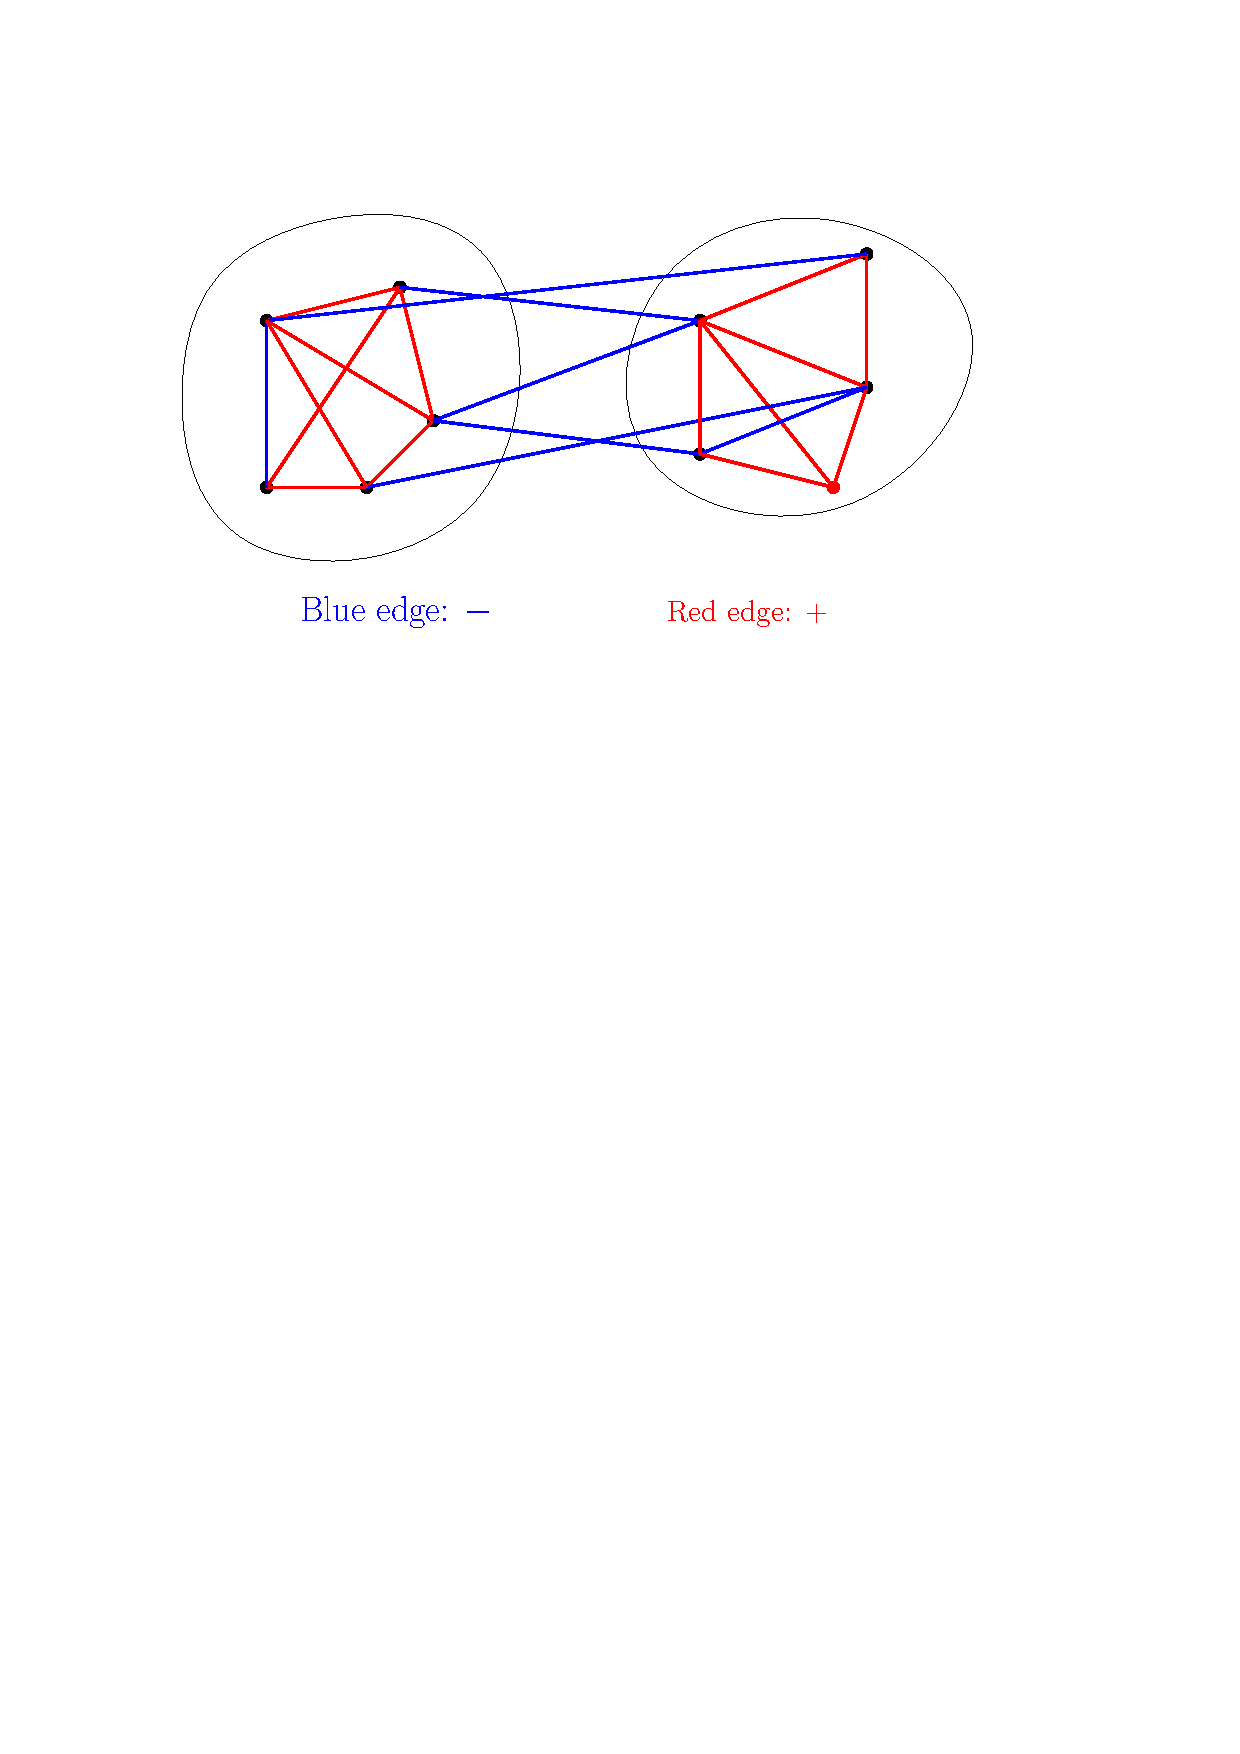
\includegraphics[scale=0.4]{Source/signed_graph.pdf}
\end{figure}
\mypv 

\vspace{-4mm}
\textbf{Goal}: 

%\begin{itemize}
%\item 
Maximize the sum of weights of: \red{intra cluster positive edges} plus \blue{inter cluster  negative  edges}  % , or 
% \item Minimize sum of weights of: inter cluster \textcolor{red}{$+$} edges plus intra cluster \textcolor{blue}{$-$} edges
% \end{itemize}
\vfill 
\end{frame}



%%%%%%%%%%%%%%%%%%%%%%%%%%%%%%%%%%%%%%%%%%%%%%%%%%%%%%%%%%%%
\begin{frame}{Signed clustering literature}

\vfill


\begin{itemize}
% \item  clustering, link prediction, visualization of signed graphs
% \mypv
\item Kunegis et al. (2010)  solved a signed version of the 2-way ratio-cut problem  via the Signed (combinatorial) graph Laplacian $ \bar{L} = \bar{D} - A$.   

\begin{itemize}   
\item the \red{random-walk normalized Laplacian}
% \vspace{-2mm}
% \begin{equation}
$ \bar{L}_{\text{rw}} = I - \bar{D}^{-1} A $ 


\item  the \red{symmetric graph Laplacian} 
$  \bar{L}_{\text{sym}} = I - \bar{D}^{-1/2} A \bar{D}^{-1/2} $ 
(skewed deg dist)
\end{itemize}

\item  Top (eigenvalues, eigenvectors) of the Signed Laplacians contain information on  the topological structure of the network. No theoretical recovery guarantees. 
\end{itemize}

\mypv  
% Once \(\mathcal{G}\) is obtained, the following clustering algorithms are used:


With theoretical guarantees for \blue{Signed Stochastic Block Models}:
\begin{itemize}
    \item Signed Positive Over Negative Generalized Eigenproblem (SPONGE) algorithm (\cite{cucuringuSPONGE})
    
    \item Regularized SPONGE  (\cite{cucuringuSPONGE})
\end{itemize}

\end{frame}


 
\begin{frame}
\fontsize{11pt}\selectfont
\frametitle{\large Signed clustering: a generalized eigenproblem formulation}


$H$: unsigned graph, adj. matrix $W$ ($W_{ij} > 0$) 
% with non-negative entries, 
for any cluster $C\subset V$ % we
\vspace{-2mm}
$$\Cut_{H}(C,\overline{C}) := \sum_{i\in C, j \in \overline{C} } W_{ij}$$

\vspace{-3mm}
the total weight of  edges crossing from $C$ to $\bar{C}$. %  in $H$.

\vspace{1mm}
Volume($C$): sum of degrees of nodes in $C$;  
 $\vol_H(C) = \sum_{i\in C}\sum_{j = 1}^n W_{ij}$ 

\hline 

Consider the decomposition 
\textcolor{red}{ $G = G^+ \cup  G^-$;  \quad  ($A = A^+ -  A^-$)  } 

\mypv 
\vspace{1mm}
Constrained clustering $ \Rightarrow $ minimize the two measures of  
\red{``\textit{badness}"}
\vspace{-2mm}
\red{
\begin{equation}
\label{eq:Cut_{\Gp}}
 \frac{\Cut_{\Gp}(C,\overline{C})}{\vol_{\Gp}(C)},
\end{equation} 
}
% \myp
\vspace{-2mm}
\begin{equation}\label{eq:Cut_{\Gn}}
 \Big( \frac{\Cut_{\Gn}(C,\overline{C})}{\vol_{\Gn}(C)} \Big)^{-1} = \red{\frac{\vol_{\Gn}(C)}{\Cut_{\Gn}(C,\overline{C})}}. 
\end{equation}
\vspace{-2mm}


 \mypv
Ideally, want $C$ s.t.   both~\eqref{eq:Cut_{\Gp}} and~\eqref{eq:Cut_{\Gn}} are small. 
% \mypv 
``Merge'' obj.~\eqref{eq:Cut_{\Gp}}+\eqref{eq:Cut_{\Gn}} 
\vspace{-3mm}
\begin{equation}\label{eq:objective_function}
\min_{C\subset V}\,\, \frac{\Cut_{\Gp}(C,\overline{C}) +  \taun \vol_{\Gn}(C)}{ \Cut_{\Gn}(C,\overline{C}) +   \taup \vol_{\Gp}(C) }, 
\end{equation}
\vspace{-3mm}

$ \taup, \taun > 0$ denote trade-off/regularization parameters.
   
\end{frame}
 



\begin{frame}
\fontsize{11pt}\selectfont
% % \red{$\vardiamond$}  
\frametitle{\large Signed clustering: a generalized eigenproblem formulation (SPONGE)}
 
Natural extension to  % the case 
$k > 2$ disjoint clusters $C_1,\hdots,C_k$ 
% leads to the following discrete optimization  problem

\vspace{-1mm}
\begin{equation}
\label{eq:discrete_optimization_problem}
\min_{C_1,\hdots,C_k} \sum_{i=1}^k \frac{\Cut_{\Gp}(C_i,\overline{C_i}) + \taun  \vol_{\Gn}(C_i)}{\Cut_{\Gn}(C_i,\overline{C_i}) + \taup \vol_{\Gp}(C_i)}.
\end{equation}
\vspace{-2mm}
% \mypv 

% Given a subset $C_i\subset V$ we can define a normalized indicator vector $x_{C_i}$
For a subset $C_i\subset V$, the normalized indicator vector % is % $x_{C_i}$

\vspace{-2mm}
\begin{equation}
(x_{C_i})_j = 
 \begin{cases} 
(\Cut_{\Gn}(C_i,\overline{C_i}) + \vol_{\Gp}(C_i))^{-1/2} ; & v_j \in C_i \\
0 ; &  v_j \notin C_i
\end{cases}
\end{equation}
\vspace{-2mm}

% \mypv 
renders~\eqref{eq:discrete_optimization_problem} % to be rewritten 
as the  discrete optimization problem

\textcolor{red}{
\vspace{-2mm}
\begin{equation}
\label{eq:discrete_optimization_problem-2}
\min_{C_1,\hdots,C_k} \sum_{i=1}^k \frac{ x_{C_i}^T (\Lp +  \taun \Dn) x_{C_i} }{ x_{C_i}^T (\Ln +  \taup \Dp) x_{C_i} }, 
\end{equation}
} 
\vspace{-2mm}

% \mypv 
which is NP-hard. 

\begin{itemize}
\item $\Lp$ (resp. $\Ln$): Laplacian of $\Gp$ (resp. $\Gn$)
\item $\Dp$ (resp. $\Dn$): diagonal matrix with the degrees of $\Gp$ (resp. $\Gn$)
\end{itemize}

\end{frame}% 





\begin{frame}
\frametitle{\large  Signed clustering: a generalized eigenproblem formulation (SPONGE)}

% A common approach: 
\red{Relaxation:} Drop the discreteness constraint  \& allow each $x_{C_i}$  % to take values in 
$\in  \mathbb{R}^n$
\begin{itemize}
\item new set of vectors $z_1,\ldots,z_k\in\mathbb{R}^n$ % that are 
orthonormal w.r.t. $\Ln+ \taup \Dp$ 

\vspace{0mm}
\begin{itemize}
  \setlength\itemsep{0em}
 \item $z_i^T  (\Ln  +   \taup  \Dp) z_i =1$, and 
 \item $z_i(\Ln + \taup   \Dp)z_j= 0$, for $i \neq j$
\end{itemize}
\vspace{-1mm}

% --------    
% \myp 
% leading to the following modified version of
leads to the following modified version of \eqref{eq:discrete_optimization_problem-2}  

\vspace{-3mm}
\begin{equation}\label{eq:discrete_optimization_problem-z}
 \min_{z_i(\Ln+\Dp)z_j=\delta_{ij}} \sum_{i=1}^k \frac{ z_i^T (\Lp + \taun  \Dn) z_i }{ z_i^T (\Ln + \taup  \Dp) z_i }.
\end{equation}
\vspace{-2mm}

\myp 
% --------   \myp 
% Note  % that 
\item % the above 
choice of $(\Ln  +   \taup  \Dp) $-orthonormality of vectors $z_1,\ldots,z_k$ 
% with respect to $\Ln+\Dp$ 
is not 
% -- strictly speaking -- 
a relaxation of \eqref{eq:discrete_optimization_problem-2};  
leads to a \red{suitable eigenvalue problem} 

% --------    
\mypv 
\item assuming $\Ln +  \taup  \Dp$ full rank, consider the change of variables 

\vspace{-4mm}
\begin{equation}
y_i=(\Ln +  \taup  \Dp)^{1/2}z_i,   
\end{equation}
\vspace{-6mm}

\item changes the orthonormality constraints of~\eqref{eq:discrete_optimization_problem-2}
to  $y_i^T y_j = \delta_{ij}$. 

% \myp 
\item   denoting matrix $Y=[y_1,\ldots,y_k ]\in\mathbb{R}^{n\times k}$, one can rewrite~\eqref{eq:discrete_optimization_problem-z} as 

  
\textcolor{red}{ 
\vspace{-3mm}
% \hspace{-3mm}
\begin{align}
\label{eq:discrete_optimization_problem_y__}
\hspace{-14mm}
 \min_{Y^T Y = I}  \Tr \Big( Y^T  \textcolor{blue}{ (\Ln + \taup \Dp)^{-1/2}   (\Lp + \taun \Dn) (\Ln + \taup \Dp)^{-1/2} }  Y  \Big)  
 % \nonumber
\end{align}
\vspace{-3mm}
}

\mypv
\item solution: eigenvectors to the $k$-smallest eigenvalues of 
\textcolor{blue}{$$ T = (\Ln +  \taup \Dp)^{-1/2}  (\Lp +  \taun \Dn) (\Ln +  \taup \Dp)^{-1/2}$$}  
% (see for eg. \cite[Theorem 2.1]{sameh2000}). 
 
%One can also verify that $(\lambda,v)$ is an eigenpair of the previous matrix if and only 
%if $(\lambda, (\Ln +  \taup \Dp)^{-1/2}v)$ is a \emph{generalized} eigenpair of 
%$( \Lp +  \taun \Dn, \Ln +  \taup \Dp)$. 

\end{itemize}

\end{frame}






%\mypv 

%\vfill 
%\end{frame}
%%%%%%%%%%%%%%%%%%%%%%%%%%%%%%%%%%%%%%%%%%%%%%%%%%%%%%%%%%%


\section{Trading strategy framework}
\label{trading-strat}
%%%%%%%%%%%%%%%%%%%%%%%%%%%%%%%%%%%%%%%%%%%%%%%%%%%%%%%%%%%%
\begin{frame}{Trading strategy implementation}

    \textbf{Objective:} Develop a trading strategy using the previous approach to demonstrate its \red{economic benefits}.

    \centering 
    
\vfill 

    \textbf{Outline:}
    \begin{enumerate}
        \item Define and implement the strategy,
        \item Evaluate its performance through backtesting.
    \end{enumerate}

\vfill 

    \begin{table}[h]
    \centering
    \begin{tabular}{ll}
        \toprule
        \textbf{Parameter} & \textbf{Description} \\
        \midrule
        \textit{Size of the asset universe} & \( n \in \mathbb{N} \) \\
        \textit{Number of clusters} & \( K \in \mathbb{N} \) \\
        \textit{Lookback window} & \( L \in \mathbb{N} \) \\
        \textit{Evaluation window} & \( s \in \mathbb{N} \) \\
        \textit{Ensembling count} & \( R \in \mathbb{N} \) \\
        \bottomrule
    \end{tabular}
    \caption{Main parameters for the strategy.}
    \label{tab:parameters}
    \end{table}

\end{frame}


\begin{frame}{Pipeline }
\label{general-setting-strat}


    \begin{enumerate}
    \item[(i)] \textbf{CLUSTERING}: 
    cluster assets based on historical returns with a lookback window of $L$ trading days (i.e. on $\Tilde{\mathbf{r}}^{(i)} \in \mathbb{R}^L$).
        \begin{enumerate}
            \item[$\bullet$] \textbf{Input}: asset returns  on $L$ days $\Tilde{\mathbf{r}}^{(1)}, \hdots, \Tilde{\mathbf{r}}^{(i)}$,
            \item[$\bullet$] \textbf{Output}: vector of cluster labels $A \in \mathbb{R}^{n}$ where $A^{(i)} \in \{1, \hdots, K\}$ is the label of the $i$-th asset cluster. 
        \end{enumerate}

\mypv 
    \item[(ii)] \textbf{PORTFOLIO CONSTRUCTION PHASE}: For each cluster $k \in \{1, \ldots, K\}$, compute the following in order:
        \begin{enumerate}
            \item[(a)] \textit{Intra-cluster weights} \((\beta_{i,k})\) for each asset in each cluster
            \item[(b)] For each cluster
            \begin{itemize}
                \item \textit{return} $r^*_k = \sum_{i=1}^n \beta_{i,k} r_i \mathbf{1}_{(A^{(i)}=k)}$ of the cluster
                \item \textit{expected return} $\bar{r}^*_k = \sum_{i=1}^n \beta_{i,k} \bar{r}_i \mathbf{1}_{(A^{(i)}=k)}$
                \item \textit{covariance matrix} $\boldsymbol{\Sigma}^*= (\text{cov}(r^*_k, r^*_l))_{1 \leq k,l \leq K}$
            \end{itemize}
            \item[(c)] \textit{Extra-cluster weights} \(\alpha_1, \ldots, \alpha_K\) are the Markowitz portfolio weights for each cluster computed using $\boldsymbol{\Sigma}^*$, $\bar{r}^*_k$'s and $r^*_k$'s.
        \end{enumerate}
    \begin{enumerate}
        \item[$\bullet$] \textbf{Input}: vector of cluster labels $A \in \mathbb{R}^n$;
        \item[$\bullet$] \textbf{Output}: weight vector (\textit{i.e.} portfolio) $\bm{\omega} = [\omega_1, \hdots, \omega_n]^T$, where $\omega_i =\alpha_{A^{(i)}}\beta_{i, A^{(i)}}$ \\
    \end{enumerate}
    \end{enumerate}

\vfill 

\end{frame}
%%%%%%%%%%%%%%%%%%%%%%%%%%%%%%%%%%%%%%%%%%%%%%%%%%%%%%%%%%%%

\begin{frame}{Pipeline}
\vfill 

    \begin{enumerate}
    \item[(iii)] \textbf{ROBUSTNESS/ENSEMBLING}: Iterate phases (1) and (2) \( R \) times \textit{within the same time frame} \([t-L; t]\) to minimize variability caused by the randomness of clustering methods (\textit{e.g.}, k-means in SPONGE).
    \begin{enumerate}
        \item[$\bullet$] \textbf{Input}: \( R \) portfolios \(\bm{\omega}_1, \ldots, \bm{\omega}_R\) (outputs from phase (2));
        \item[$\bullet$] \textbf{Outcome}: Final portfolio \(\boldsymbol{\omega}_{mean} = \frac{1}{R} \sum_{r=1}^R \bm{\omega}_r \in \mathbb{R}^n\), calculated as the mean of the portfolios across all runs.
    \end{enumerate}
       
    \mypv 
       
    \item[(iv)] \textbf{EVALUATION PHASE}: Initiate the portfolio with long/short positions in each constituent, and hold these positions for the \textit{evaluation window} \([t; t+s]\), where \(s\) is the window length.
    \end{enumerate}
\centering 

\vfill 
\end{frame}


\begin{frame}{Pipeline}
\centering
\begin{figure}
        \centering
        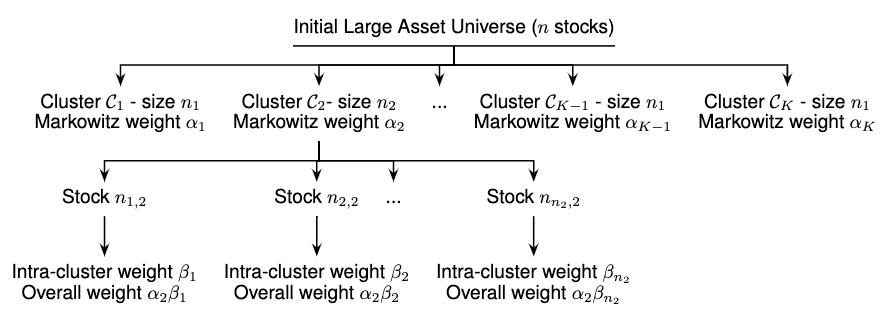
\includegraphics[width=0.85\linewidth]{Source/three.png}
        \vspace{-3mm}
        \caption{Illustration of phase (i) and (ii)}
        \label{weights-relationship}
\end{figure} 

% \vspace{0.2cm}
\mypv 

\begin{figure}[H]
    \centering
    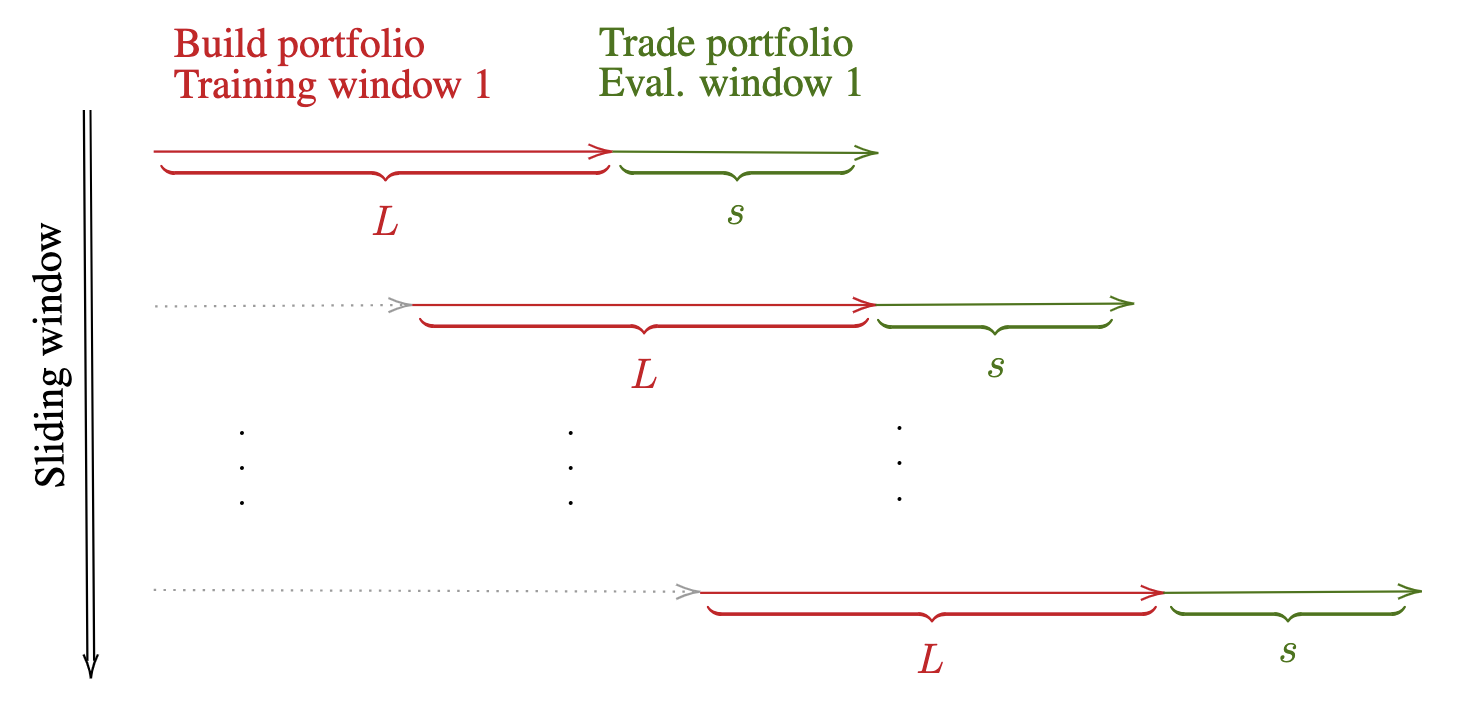
\includegraphics[width=0.45\linewidth]{Source/strat.png}
    \vspace{-2mm}
    \caption{Representation of the walk-forward train-test split of the  strategy.}
    \label{sliding-window-representation}
\end{figure}

% \mypv 

\vfill 
\end{frame}


% \ section{Discussion on key parameters}
\section{Parameters}

%%%%%%%%%%%%%%%%%%%%%%%%%%%%%%%%%%%%%%%%%%%%%%%%%%%%%%%%%%%%
\begin{frame}{Gaussian constituent weights}

    \textbf{Intra-cluster weights (\( \beta_{i,k} \)) via a Gaussian Kernel}

    \vspace{0.2cm}

    \textbf{Objective:} Assign intra-cluster weights to assets based on their proximity to the cluster centroid \( \mu_k \) (defined as the mean return vector of assets in \( \mathcal{C}_k \))

   \begin{equation}
    \beta_{i_k} = \frac{\exp\left(-\frac{\lVert \mathbf{r}^{(i)} - \mu_k \rVert^2}{2\sigma^2}\right)}{\sum_{j \in \mathcal{C}_k} \exp\left(-\frac{\lVert \mathbf{r}^{(j)} - \mu_k \rVert^2}{2\sigma^2}\right)}
   \end{equation}
where
    \begin{itemize}
        \item \( \sigma^2 \) is the Kernel bandwidth (controls dispersion;  optimized by cross-validation)  
    \end{itemize}

%    \vspace{0.2cm}
\mypv 

 \textbf{Key Benefits:}
    \begin{itemize}
        \item Ensures all assets in a cluster contribute, rather than selecting a single representative.
        \item Enhances cluster distinctions while maintaining diversification.
    \end{itemize}
    \vfill
\end{frame}
%%%%%%%%%%%%%%%%%%%%%%%%%%%%%%%%%%%%%%%%%%%%%%%%%%%%%%%%%%%%



%%%%%%%%%%%%%%%%%%%%%%%%%%%%%%%%%%%%%%%%%%%%%%%%%%%%%%%%%%%%
\begin{frame}{Synthetic returns for the Markowitz optimization}
% Estimation of returns
\footnotesize

\textbf{Objective:} Simulate forecasted returns for clusters

    \vspace{0.2cm}

    \textbf{Procedure:}
    \begin{itemize}
        \item Portfolio is constructed at time \( t \) and held over the period \([t, t+s]\).
        \item For each cluster \( k \), let \(\textbf{y}_k \in \mathbb{R}^{s}\) represent the true vector of its future returns over \( s \) evaluation days.
    \end{itemize}

\mypv 

    \textbf{Simulation of noisy forecasts} 
    \begin{itemize}
        \item To simulate forecast accuracy, add noise to \(\textbf{y}_k\) to create \(\hat{\textbf{y}}_k = \textbf{y}_k + \epsilon_k\), where \(\epsilon_k \sim \mathcal{N}(0, \sigma_{\eta}^2 I_s)\).
        \item The noise level \( \sigma_{\eta} \) is adjusted to reach an average empirical correlation \(\eta\) between \(\textbf{y}_k\) and \(\hat{\textbf{y}}_k\).
    \end{itemize}

\mypv 

    \textbf{Achieving target correlation}
    \[
    \frac{1}{K} \sum_{k=1}^K \widehat{\text{corr}}(\textbf{y}_k, \hat{\textbf{y}}_k) = \eta
    \]
    \begin{itemize}
        \item Noise level \( \sigma_{\eta} \) is iteratively adjusted until this target correlation is met.
    \end{itemize}

    \vfill

\end{frame}
%%%%%%%%%%%%%%%%%%%%%%%%%%%%%%%%%%%%%%%%%%%%%%%%%%%%%%%%%%%%







\begin{frame}{Optimal number of clusters}

    \textbf{Objective:} Identify the smallest number of clusters/components \( K \), that explains a significant proportion of the variance in the data.

    \begin{itemize}
        \item Set a threshold \( P \) and find the smallest \( k \) such that:$
            \frac{\sum_{i=1}^{k} \lambda_i}{\sum_{i=1}^{n} \lambda_i} \geq P
        $
    \end{itemize}

    \vspace{0.4cm}

    \begin{columns}
        \column{0.5\textwidth}
        \begin{figure}
            \centering
            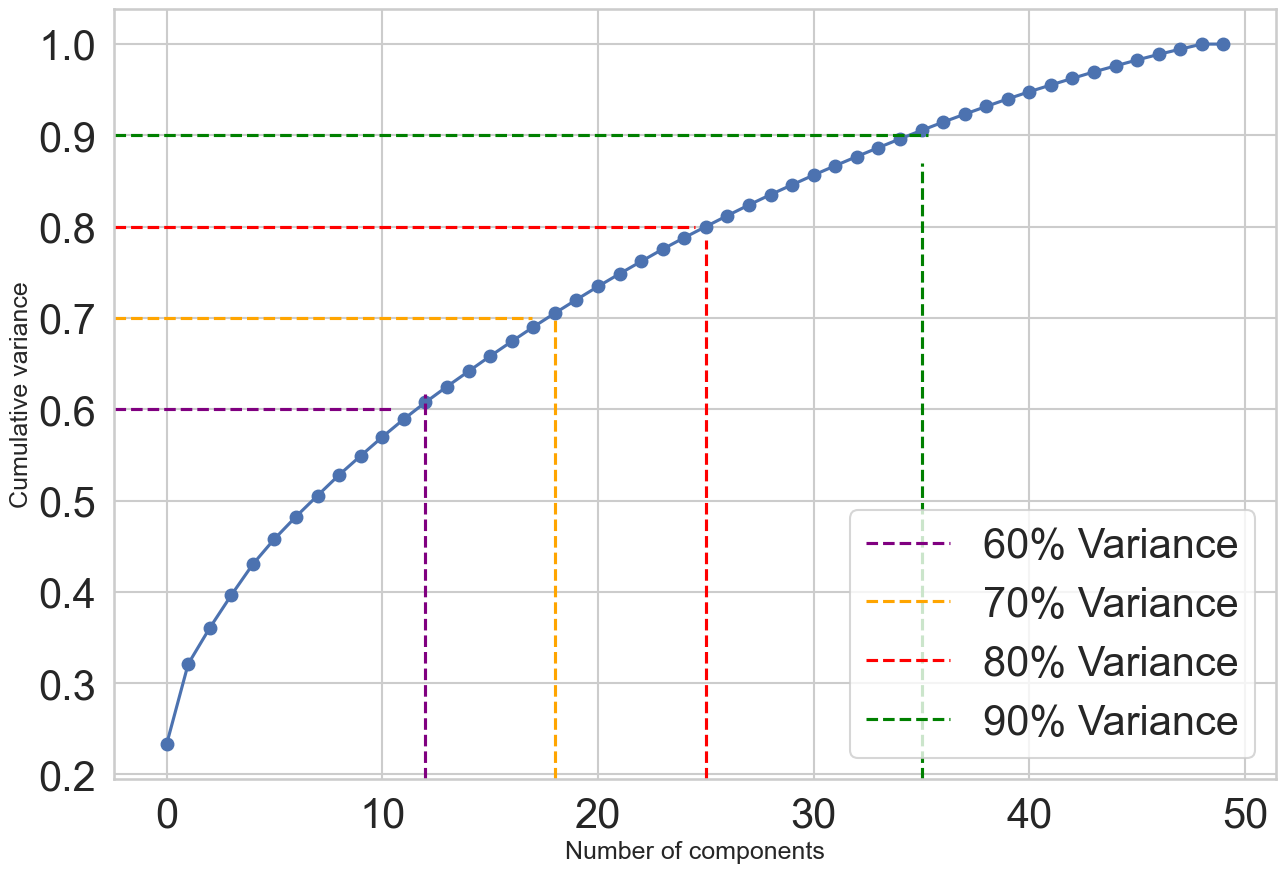
\includegraphics[width=\textwidth]{Source/PCA.png} % Remplacez 'PCA.png' par le fichier de l'image réelle
            \caption{PCA Analysis - Cumulative Variance Explained}
            \label{fig:pca}
        \end{figure}

        \column{0.5\textwidth}
        \textbf{Key Findings:}
        \begin{itemize}
            \item \red{Considering  60\% and 80\% of explained variance, two cluster counts (10 and 24) stand out}
            \item These correspond to levels in the \blue{Global Industry Classification Standard (GICS®):10 sectors and 24 industry groups}
        \end{itemize}
    \end{columns}

\end{frame}



\begin{frame}{Turnover and transaction costs}
\footnotesize
    \centering

    \begin{itemize}
        \item Vary transaction costs in 1 bpts increments.
        % A transaction rate of 0.01\% is set.
    \end{itemize}

    \vspace{0.1cm}

    \begin{columns}
        \column{0.47\textwidth}
        \textbf{Observations:}
        \begin{itemize}
            \item Transaction costs have a larger impact at daily frequency.
            \item Daily strategy outperforms naive Markowitz up to 13 basis points.
            \item Weekly strategy outperforms naive Markowitz up to 18 basis points.
        \end{itemize}

        \column{0.55\textwidth}
        \begin{figure}
            \centering
            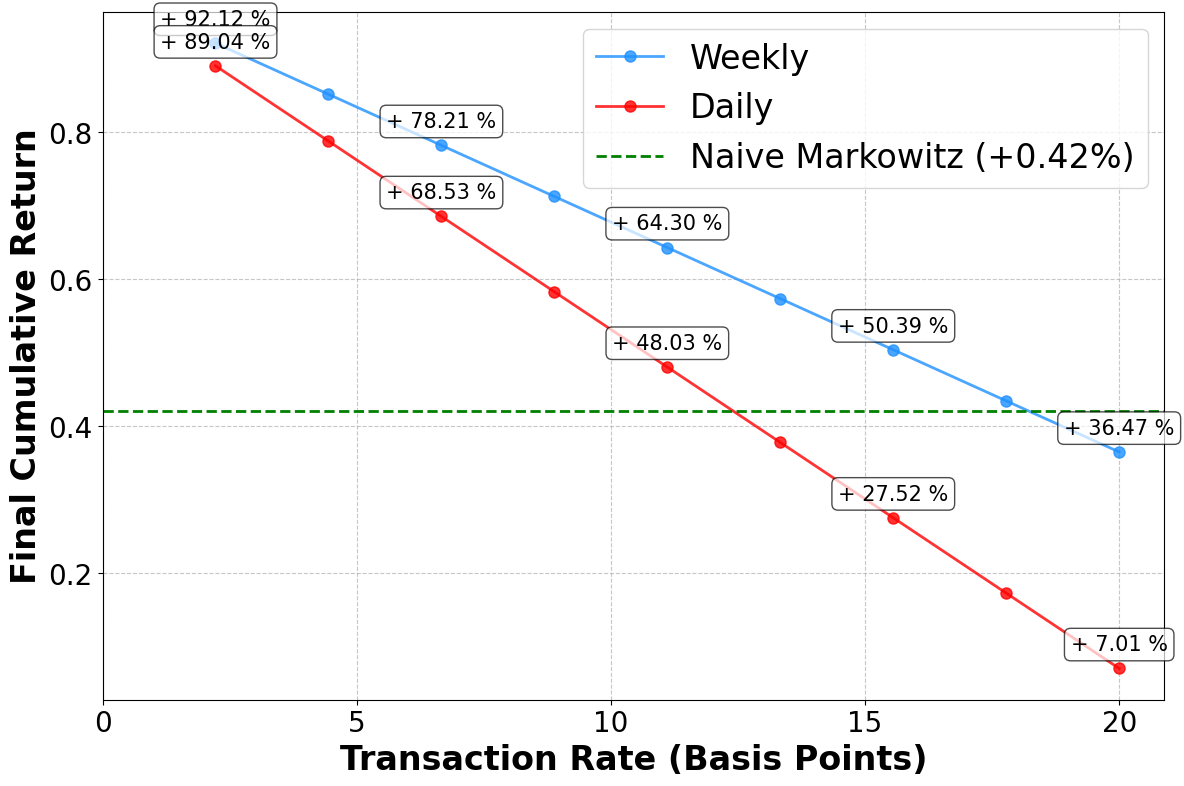
\includegraphics[width=\textwidth]{Source/transac_cost_impact.png} % Replace 'transac_cost_impact.png' with your actual image file
            \caption{Impact of transaction costs on cumulative returns}
            \label{transac-cost-impact}
        \end{figure}
    \end{columns}

\end{frame}



\begin{frame}{EWA covariance matrix: addressing non-stationarity}
\footnotesize

    \textbf{Motivation:}
    \begin{itemize}
        \item Financial returns often exhibit \textit{volatility clustering} (\cite{Mandelbrot}) that can lead to reduced effective sample size in volatile periods, calling for a method that adjusts for \blue{non-stationary environments}
    \end{itemize}

\mypv

    \textbf{Solution: \red{Exponentially Weighted Average} (EWA) Covariance Matrix}
    \begin{itemize}
        \item EWA schemes are suitable for non-stationary, heteroskedastic environment by emphasizing more recent observations.
        \item Denoting the matrix of observations by $\bm{X} = \begin{bmatrix} \mathbf{r}^{(1)} | \hdots |\mathbf{r}^{(n)}\end{bmatrix} \in \mathbb{R}^{d \times n}$ and assuming returns to centered, the EWA sample covariance matrix (\cite{TanZohren}) is defined as
        \[
        \bm{E} := \frac{1 - \beta}{1 - \beta^d} \sum_{t=1}^{d} \beta^{d-t} r_t^T r_t
        \]
        where \( \beta \in (0, 1) \) is the \textit{exponential decay rate}.
    \end{itemize}

\mypv 
    
    \textbf{Decay Rate Impact:}
    \begin{itemize}
        \item As \( \beta \to 1 \): EWA converges to the standard covariance matrix.
        \item As \( \beta \) decreases, recent data is weighted more heavily, enhancing responsiveness to recent volatility changes.
    \end{itemize}

\end{frame}
%%%%%%%%%%%%%%%%%%%%%%%%%%%%%%%%%%%%%%%%%%%%%%%%%%%%%%%%%%%%




\section{Empirical results}
\label{empirical}

% The framework outlined in Section \ref{trading-strat} is subjected to back-testing on a large universe of assets of $n=695$ stocks for which we have daily data available every day for the entire duration of the study (refer to database \cite{WhartonDATA}, which includes daily returns of NYSE stocks from January 2013 to December 2019). The four trading strategies—named after the respective clustering algorithms—are compared with each other as well as with so-called \textit{naive} strategies. These strategies are highly sensitive to their underlying parameters, specifically $\eta$, representing prediction quality, and $K$, the number of clusters. The back-testing is conducted by simulating a portfolio that initially invested \$1 on January 1, 2013, with \$1 reinvested at each trading period based on the evaluation window. In all subsequent simulations, parameter values are fixed as detailed in Table \ref{params}. The number of clusters, \( K \), and the prediction level, $\eta$, are varied across the sets $K \in \{10, 17, 24\}$ and $\eta \in \{0, 0.01, 0.1, 0.5, 0.9, 1\}$, respectively, to evaluate the sensitivity of the strategy to these parameters.

 \begin{frame}{Backtesting framework}
    \begin{itemize}
        \item \textbf{Asset universe:} Tested on $n=695$ NYSE stocks, with daily data from January 2013 to December 2019 (\cite{WhartonDATA}).

        \mypv 
        \item \textbf{Trading strategies:} Four strategies based on each clustering algorithms, compared to \textit{naive} strategies.

        \mypv 
        \item \textbf{Parameter sensitivity:}
            \begin{itemize}
                \item $\eta$: prediction quality parameter; $\eta \in \{0, 0.01, 0.1, 0.5, 0.9, 1\}$.
                \item $K$: number of clusters, tested for $K \in \{10, 17, 24\}$ (as outlined by the variance analysis).
            \end{itemize}
         \mypv    
        \item \textbf{Backtesting simulation:}
            \begin{itemize}
                \item Portfolio initialized with \$1 on January 1, 2013, reinvested every trading period based on the evaluation window.
                \item Parameters fixed as shown in Table \ref{params}.
            \end{itemize}
    \end{itemize}
    
% \mypv 

\vspace{3pt}
\begin{table}[H]
  \caption{Table of parameters}
  \label{params}
  \begin{tabular}{cccccccl}
    \toprule
     &  Lookback & $\sigma$ & Repetitions &  Eval. & $\beta$ \\
    \midrule
     & 75 trading days & 0.01 & 10 & 5 trading days& $0.9$ \\
  \bottomrule
\end{tabular}\\
\end{table}

\end{frame}





% \subsection{Naive strategies}
% In this section, three naive portfolio construction strategies that do not employ clustering are introduced. These strategies are designed to emphasize the significance of incorporating clustering into the correlation matrix prior to portfolio optimization. Let $n$ represent the number of assets in the universe. The strategies are defined as follows 

% The evolution of their respective cumulative PnL is given in Figure \ref{naivestrats-plots}.


\begin{frame}{\large Naive portfolio construction strategies}
    \begin{itemize}
        \item \textbf{Purpose:} naive benchmarks to highlight the impact of clustering.
    \end{itemize}
    
    \begin{enumerate}
        \item[(i)] \textbf{Equally-weighted portfolio:} All assets are assigned equal weights
        \[
        (\boldsymbol{\omega}_{\text{EW}, t})_i = \frac{1}{n}, \quad \forall i \in \{1, \hdots, n \}.
        \]

        \mypv 
        \item[(ii)] \textbf{Naive Markowitz strategy:} Weights optimized to minimize variance given a target return:
        \[
        (\boldsymbol{\omega}_{\text{MN}, t}) \in \arg \min_{\boldsymbol{\omega}} \left\{\boldsymbol{\omega}^T\boldsymbol{\Sigma}_t \boldsymbol{\omega} : \boldsymbol{\omega}^T \bar{r}_t  \geq \rho_{0}, \sum_{i=1}^n \omega_i = 1\right\}.
        \]
        
        % Nail:  
        % rho_0 = 0.0008 for daily returns
        % so approximately 20% annualized
\mypv 
        \item[(iii)] \textbf{S\&P500 Index strategy:} Holds an ETF that replicates the SP 500 index.
    \end{enumerate}

\mypv
These benchmarks are deliberately simplistic as the purpose of this work is to demonstrate the benefits clustering brings, rather than showing that this approach outperforms the state-of-the-art.

\end{frame}



%%%%%%%%%%%%%%%%%%%%%%%%%%%%%%%%%%%%%%%%%%%%%%%%%%%%%%%%%%%%
\begin{frame}{Naive portfolio performance}
\footnotesize
\vfill

\begin{figure}[H]
    \centering
    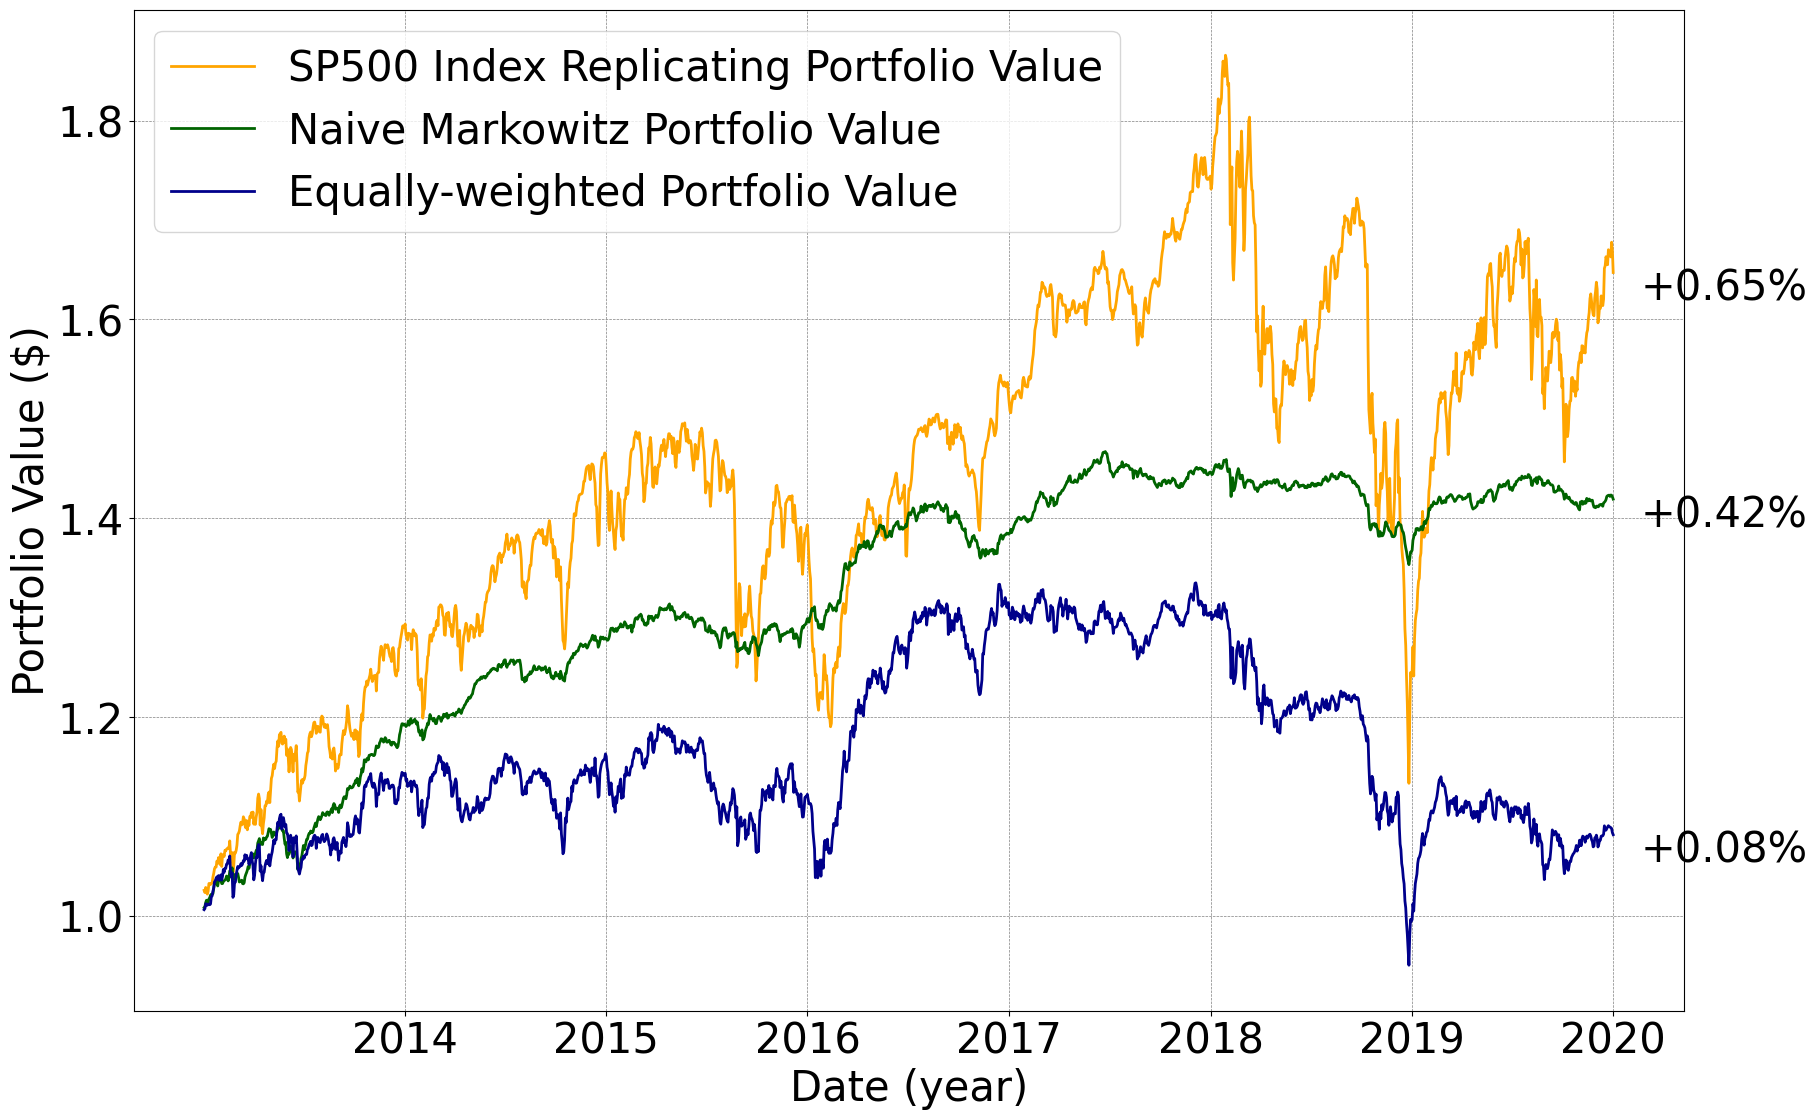
\includegraphics[width=0.55\linewidth]{Source/naive_strats.png}
    \vspace{-2mm}
    \caption{Naive portfolio values for \$1 initial investment (01-01-2013 | 31-12-2019)}
    \label{naivestrats-plots}
\end{figure}
\begin{itemize}
    \item uniform strategy performs the worst; 
    % however, there have been 
    contradicts other works 
    % such as \cite{optimal_perf_good} and \cite{optimal_porfolio_good_perf_2} which
    claiming that equally weighted strategies often outperform complex ones

    \mypv 
    \item   S\&P500 replication strategy yields the best returns at the cost of high volatility (Sharpe of 0.5)
    
    \mypv 
    \item despite the S\&P500  losing over 40\% of its value at the end of 2018, the naive Markowitz approach performed well during this downturn
\end{itemize}

\vfill 
\end{frame}
%%%%%%%%%%%%%%%%%%%%%%%%%%%%%%%%%%%%%%%%%%%%%%%%%%%%%%%%%%%%

%%%%%%%%%%%%%%%%%%%%%%%%%%%%%%%%%%%%%%%%%%%%%%%%%%%%%%%%%%%%
\begin{frame}{Clustering EWA strategies (1/2)}
   
\vfill

\begin{itemize}
    \item  performance of the four cluster-driven Markowitz strategies is compared with that of the naive Markowitz strategy

    \mypv 
    \item  cluster-based strategies consistently demonstrate superior economic performance compared to the naive approach
\end{itemize}

\mypv 

\begin{table}[H]
  \caption{Performance metrics: EWA - $K=24$ clusters and $ \eta=0.1$. Sym: SPONGE symmetric; SL: Signed Laplacian; SC: plain spectral clustering on the absolute value correlation matrix. \blue{Blue}/\red{red} denote the \blue{best}/\red{worst} performance for each metric. } 
  \label{EWA_24_perf_metrics}
  \begin{tabular}{cccccl}
    \toprule
     &  Naïve & \textbf{SPONGE} &  Sym & SL & SC\\
    \midrule
    Return & \textcolor{red}{41.92\%} & 89.36\% & 89.98\% & 86.45\% &\textcolor{blue}{91.25\%}\\ 
    AR & \textcolor{red}{5.14\%} & 9.57\% & 9.62\% & 9.33\% & \textcolor{blue}{9.73\%} \\ 
    Daily Vol. &  \textcolor{red}{0.23\%} & 0.19\% &  \textcolor{blue}{0.17\%} & 0.22\% & 0.19\% \\ 
    Annual. Vol. &  \textcolor{red}{3.59\%} & 3.09\% &  \textcolor{blue}{2.73\%} & 3.42\% &3.04\%\\ 
    Sharpe & \textcolor{red}{1.43} & 3.09 & \textcolor{blue}{3.52} & 2.72 &3.19\\ 
    Sortino & \textcolor{red}{1.97} & 4.28 & \textcolor{blue}{4.99} & 3.68& 4.33\\ 
  \bottomrule
\end{tabular}
\end{table}

\footnotesize
 
% SC is plain spectral clustering with the absolute value of the adjency matrix so that all values are positive

%SL is signed laplacian (kunegis)

%Sym is Sponge symmetric

%It is with eta = 0.1


\vfill 
\end{frame}
%%%%%%%%%%%%%%%%%%%%%%%%%%%%%%%%%%%%%%%%%%%%%%%%%%%%%%%%%%%%

%%%%%%%%%%%%%%%%%%%%%%%%%%%%%%%%%%%%%%%%%%%%%%%%%%%%%%%%%%%%
\begin{frame}{Clustering EWA strategies (2/2)}
   \footnotesize
\vfill

\begin{figure}[H]
    \centering
    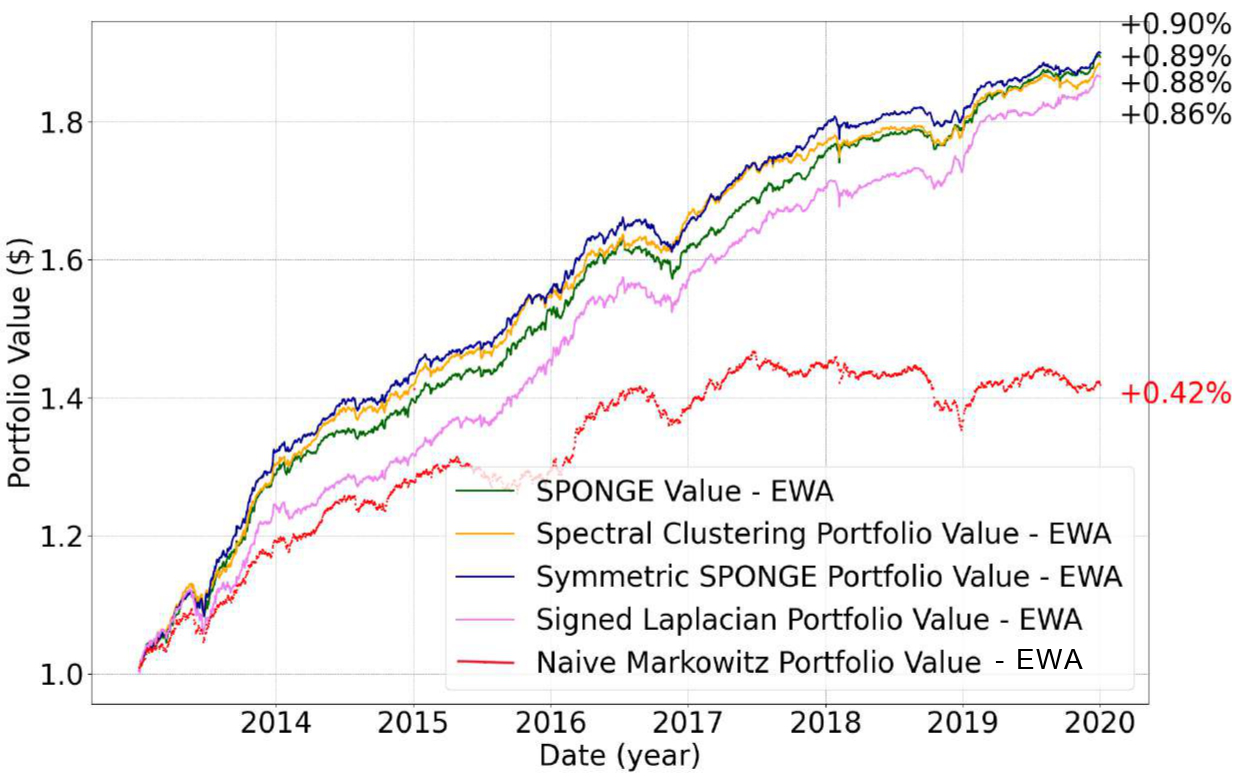
\includegraphics[width=0.55\linewidth]{Source/EWA_strats.png}
    \caption{EWA clustering vs. naive Markowitz - $K=24$ clusters.}
    \label{cumpnlstrategiesandewa}
\end{figure}

\begin{itemize}
    \item[-] \textbf{in terms of annualized and daily volatility}, the naive Markowitz strategy performs the worst; covariance estimation in a lower dimension improves performance

    \mypv 
    \item[-] \textbf{in terms of annualized return (AR)}, the clustering strategies significantly outperform the naive strategy, even in bear market conditions
\end{itemize}

\vfill 
\end{frame}
%%%%%%%%%%%%%%%%%%%%%%%%%%%%%%%%%%%%%%%%%%%%%%%%%%%%%%%%%%%%

%%%%%%%%%%%%%%%%%%%%%%%%%%%%%%%%%%%%%%%%%%%%%%%%%%%%%%%%%%%%
\begin{frame}{Performance for varying number of clusters (1/3)}
   
\vfill
\begin{itemize}
    \item The sensitivity of the strategy to the number of clusters is  assessed for $K \in \{10, 17, 24\}$ (as suggested by the explained variance), excluding EWA. 
    \mypv 
    
    \item These values are informed by the \textbf{GICS®} classification, suggesting that the cluster-driven strategies may be construed as sectorial asset trading strategies.
\end{itemize}

\vfill 
\end{frame}


\begin{frame}{\large Performance for varying number of clusters  (2/3)}
   
% \vfill
\vspace{-2mm}

\begin{figure}
\centering
% Première ligne avec deux figures
\begin{minipage}{0.435\linewidth}
  \centering
  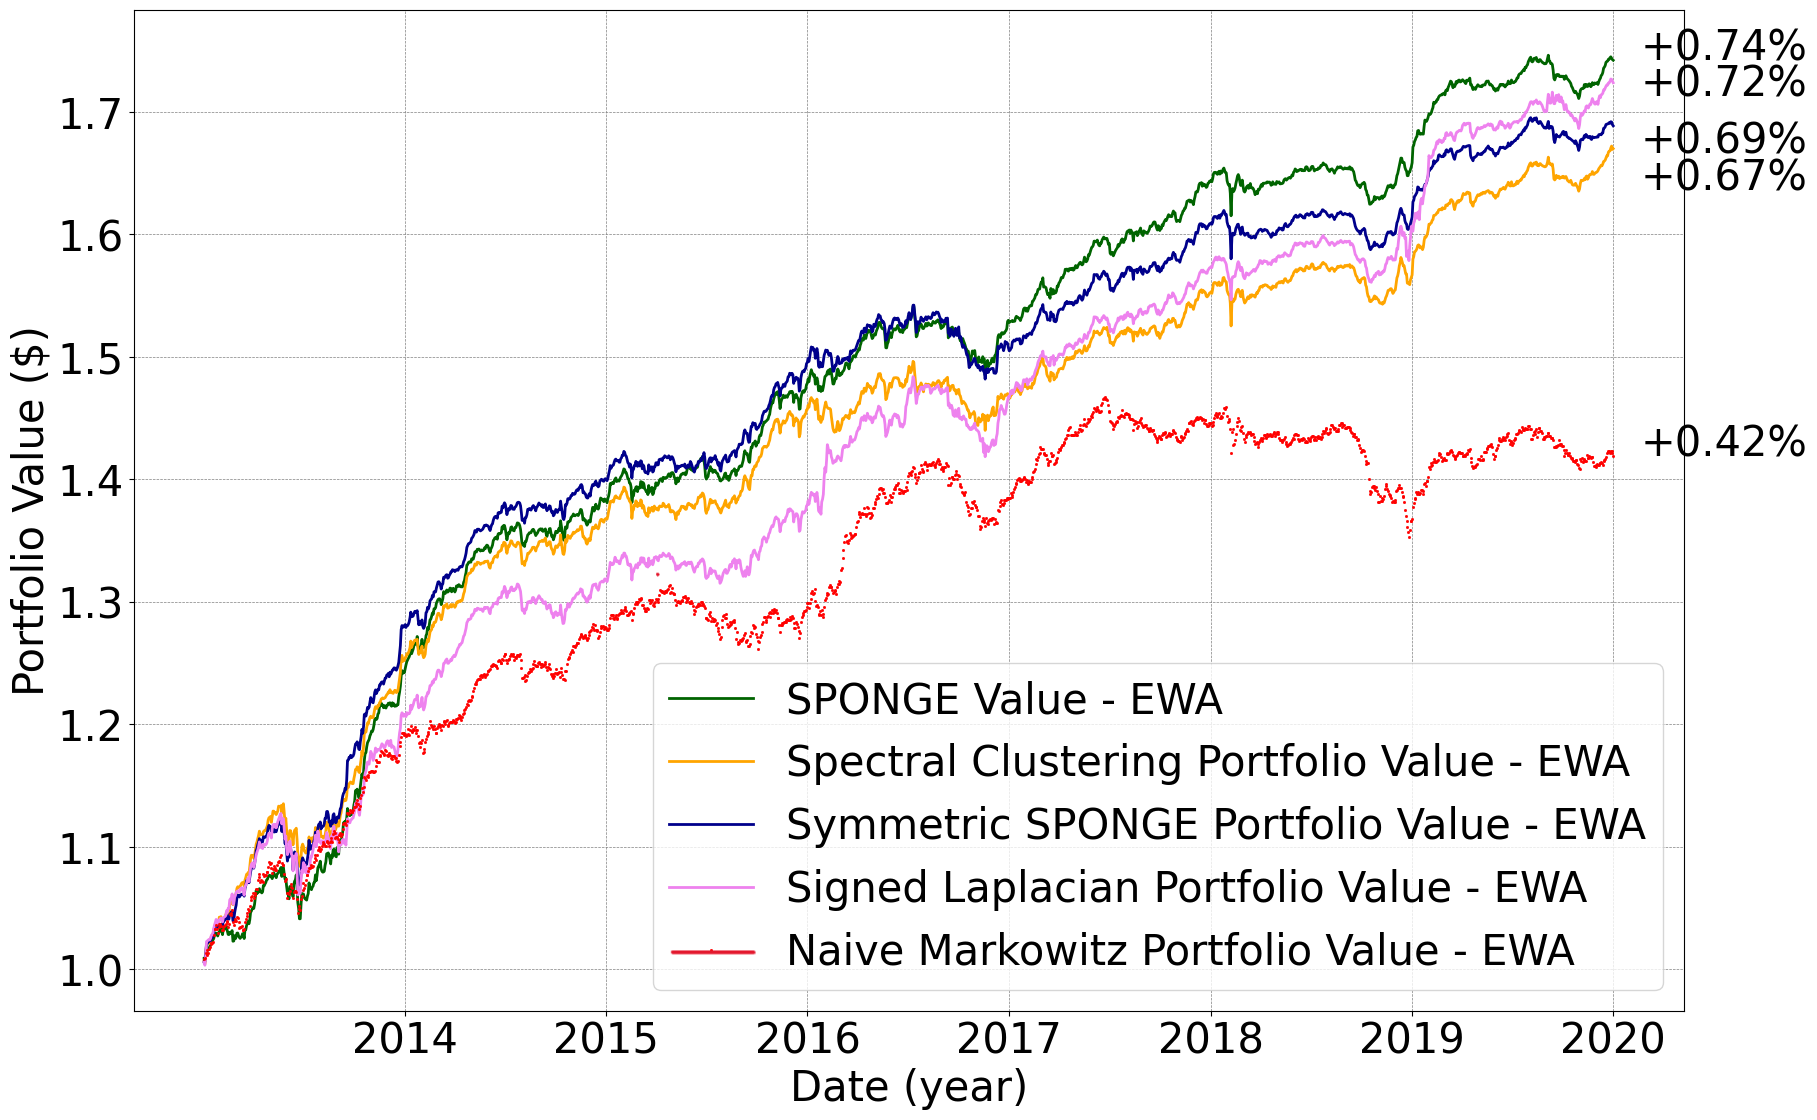
\includegraphics[width=1.0\linewidth]{Source/10_clusters_all.png}
  \caption{$K=10$; $\eta=0.10$}
  \label{10-clusters}
\end{minipage}\hfill
\begin{minipage}{0.435\linewidth}
  \centering
  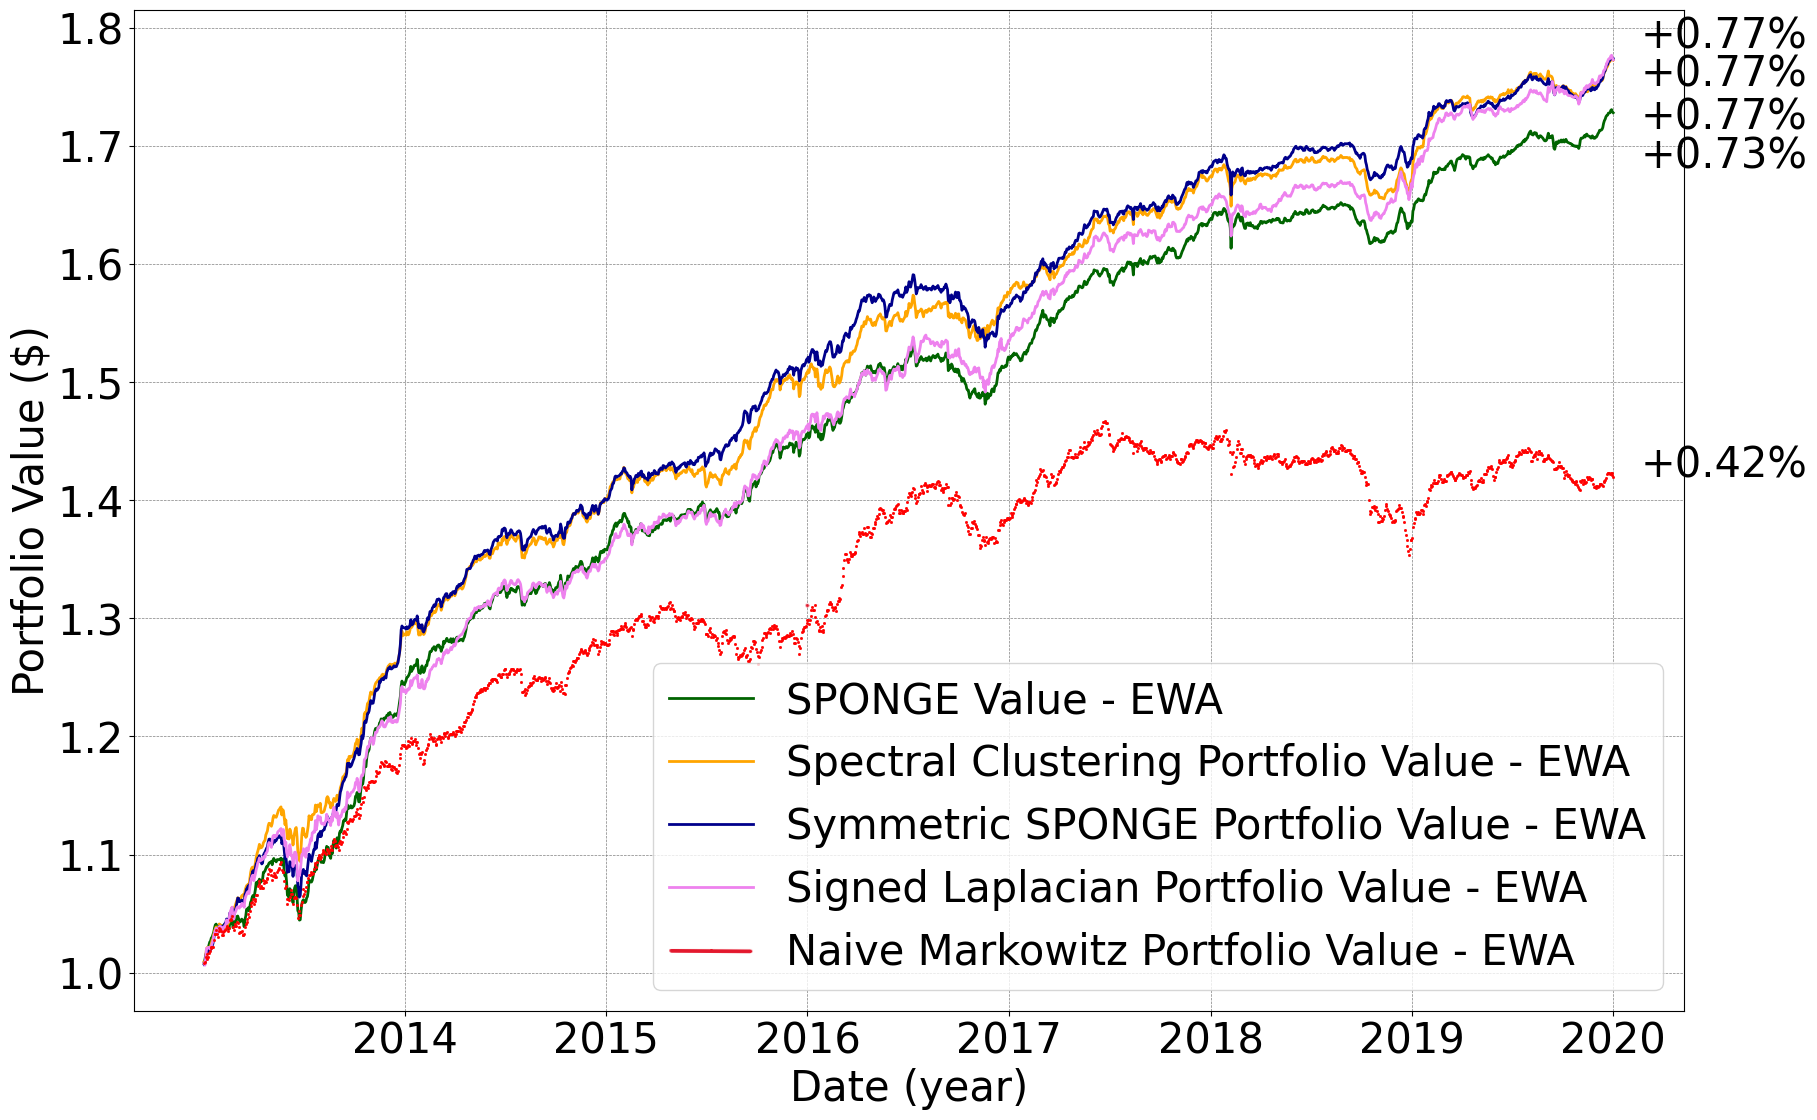
\includegraphics[width=1.0\linewidth]{Source/17_clusters_all.png}
  \caption{$K=17$, $\eta=0.10$}
  \label{17-clusters}
\end{minipage}
% Deuxième ligne avec une figure
\begin{minipage}{0.435\linewidth}
  \centering
  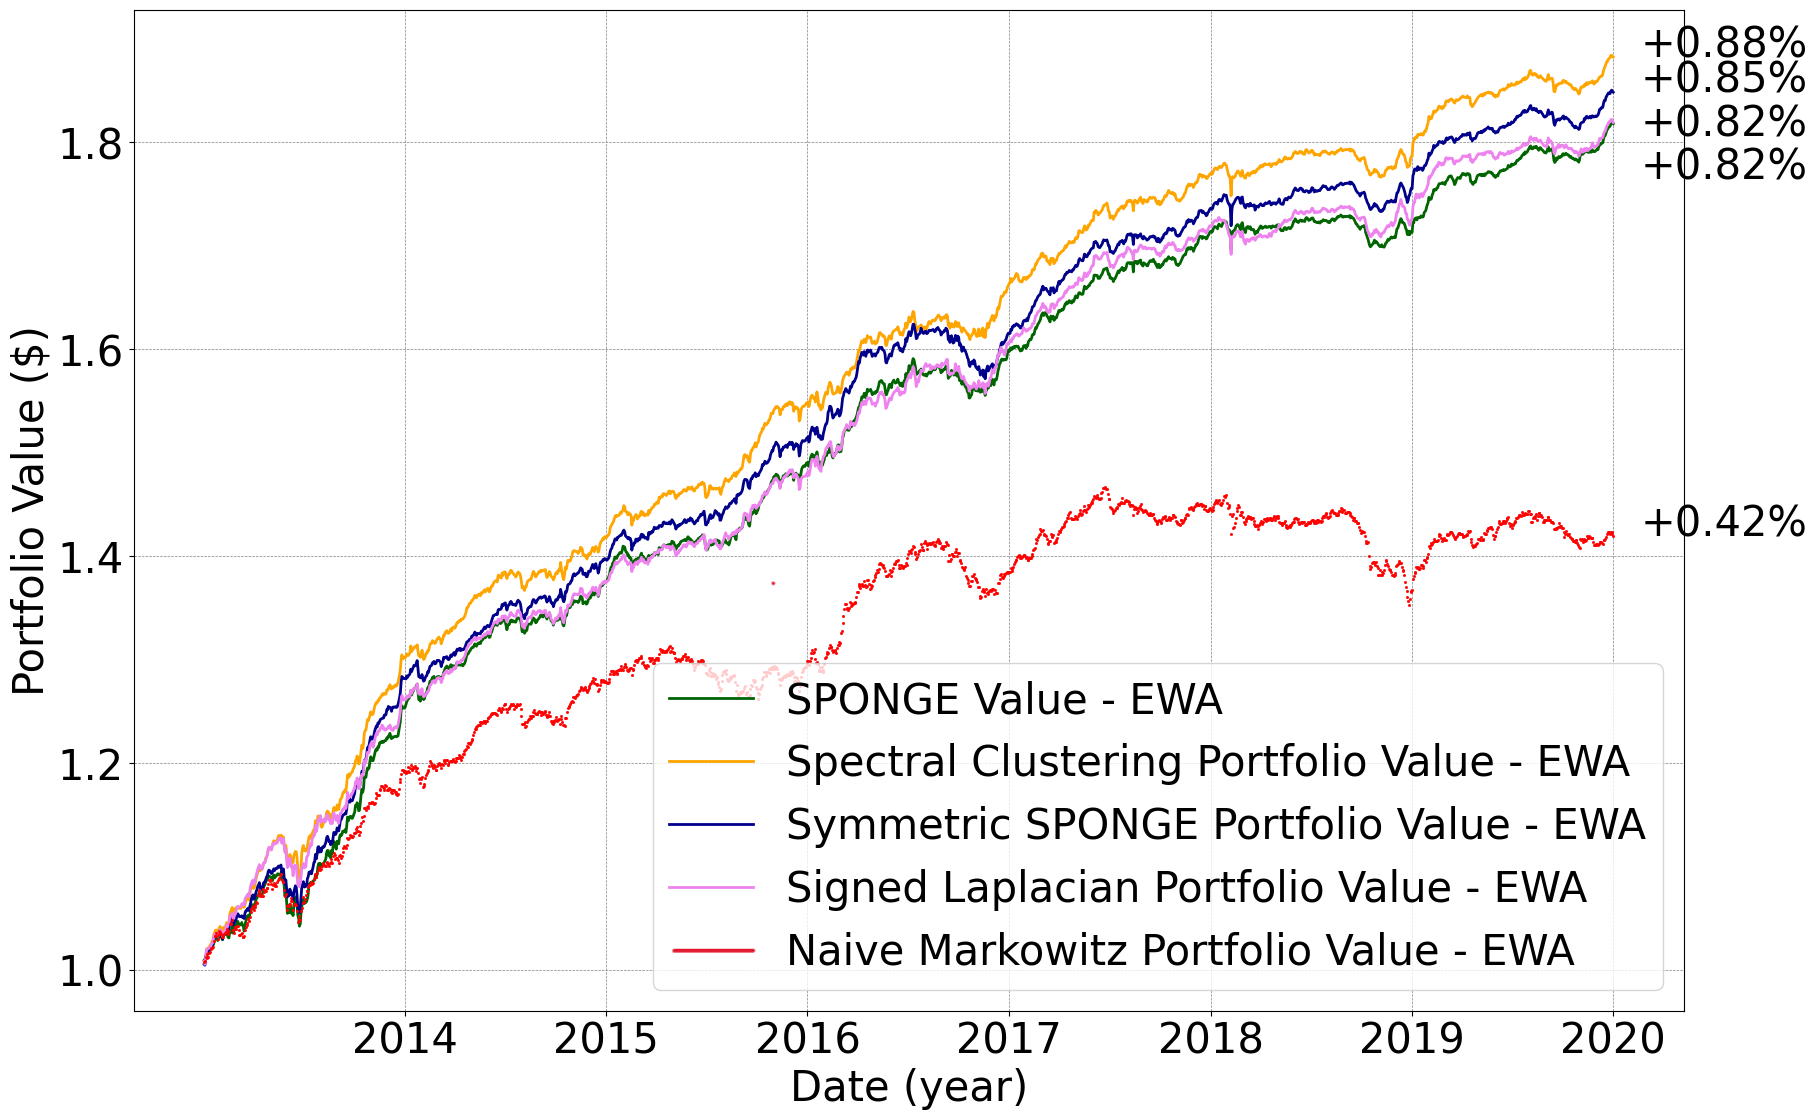
\includegraphics[width=1.0\linewidth]{Source/24-clusters.png}
  \caption{$K=24$, $\eta=0.10$}
  \label{24-clusters}
\end{minipage}

\caption{Portfolio clustering performance for varying $K$}
\end{figure}


\vfill 
\end{frame}



\begin{frame}{Performance for varying number of clusters (3/3)}
\vfill 
\begin{itemize}
    \item excluding the EWA scheme results in nearly a 10\% reduction in total return.
    
    \mypv 
    \item $K = 10$: the relatively poor results may be due to significant information loss from extensive dimensionality reduction.
    
    \mypv 
    \item   $K=17$:  performance shows slight improvement but may be influenced by limited economic interpretation
    
    \mypv 
    \item   $K=24$:  the strategy yields the \red{best results in terms of both return and volatility}; superior performance is likely due to 
       \begin{itemize}
       \item clear economic rationale behind the 24 clusters (24 industry groups in the GICS®)
       \item retention of a sufficiently high-dimensional correlation matrix that better preserves information
    \end{itemize}
    
\end{itemize}

\vfill 
\end{frame}


%%%%%%%%%%%%%%%%%%%%%%%%%%%%%%%%%%%%%%%%%%%%%%%%%%%%%%%%%%%%

%%%%%%%%%%%%%%%%%%%%%%%%%%%%%%%%%%%%%%%%%%%%%%%%%%%%%%%%%%%%
\begin{frame}{Sensitivity to the quality of the prediction $\eta$ (1/2)}
   \footnotesize
\vfill

\begin{itemize}
    \item intuitively, as $\eta$ increases, the empirical correlation between the \textit{true} vector of expected returns and its noisy counterpart also increases, enhancing the quality of predictions

    \mypv 
    \item analysis aims to illustrate how the performance of a strategy might evolve with forecast accuracy (different users have  alphas of different strengths)

    \mypv 
    \item additionally, the case  $\eta=0$ denotes that the expected return vector is simply the average return over the training period
\end{itemize}

\mypv 
\begin{table}[H]
  \caption{Performance metrics of portfolios - variations of $\eta$. \blue{Blue}/\red{red} denote the \blue{best}/\red{worst} performance for each metric.}
  \label{varying-eta-table}
  \begin{tabular}{cccccl}
    \toprule
     &  $\eta = 0.01$ & $\eta = 0.1$ &  $\eta = 0.5$ & $\eta = 0.9$ & $\eta = 1.0$\\
    \midrule
    Return & 81.39\% & \textcolor{red}{81.29\%} & 90.47\% & 116.34\% & \textcolor{blue}{205.43\%}\\
    AR & 8.90\% & \textcolor{red}{8.89\%} & 9.66\% & 11.68\% & \textcolor{blue}{17.33\%} \\
    Daily Vol. & \textcolor{red}{0.19\%} & \textcolor{red}{0.19\%} & 0.18\% & 0.17\% & \textcolor{blue}{0.14\%} \\
    Annual. Vol. & 3.04\% & \textcolor{red}{3.09\%} & 2.94\% & 2.76\% &\textcolor{blue}{2.23\%}\\
    Sharpe & 2.93 & \textcolor{red}{2.88} & 3.28 & 4.24 &\textcolor{blue}{7.76}\\
    Sortino & 3.89 & \textcolor{red}{3.75} & 4.58 & 6.00& \textcolor{blue}{12.32}\\
  \bottomrule
\end{tabular}
\end{table}
\vfill 
\end{frame}
%%%%%%%%%%%%%%%%%%%%%%%%%%%%%%%%%%%%%%%%%%%%%%%%%%%%%%%%%%%%

%%%%%%%%%%%%%%%%%%%%%%%%%%%%%%%%%%%%%%%%%%%%%%%%%%%%%%%%%%%%
\begin{frame}{Sensitivity to the quality of the prediction $\eta$ (2/2)}
\footnotesize
\vfill

\begin{figure}[H]
\centering
% Première figure
\begin{minipage}{0.45\linewidth}
  \centering
  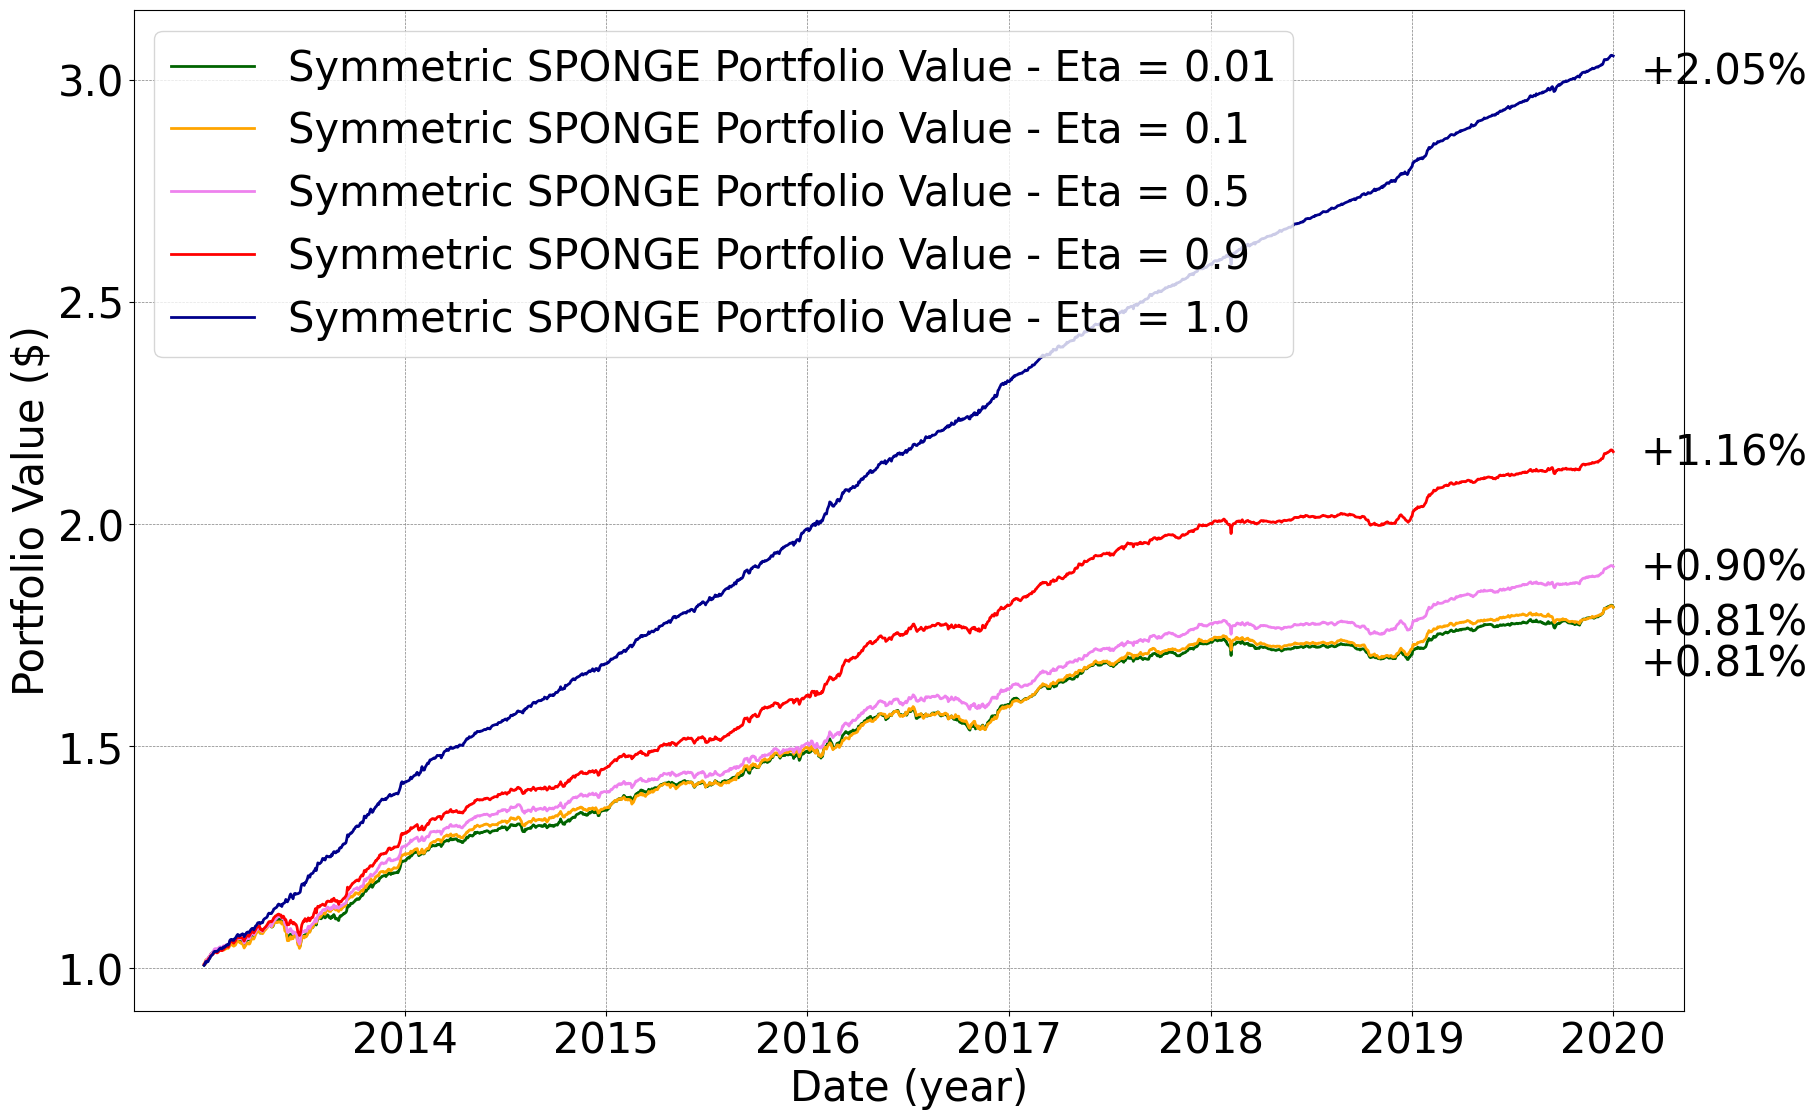
\includegraphics[width=1.0\linewidth]{Source/sponge_sym_eta_varying.png}
  \caption{$\eta \in \{0.01, 0.1, 0.5, 0.9, 1.0\}$}
  \label{varying-eta}
\end{minipage}\hfill
% Deuxième figure
\begin{minipage}{0.45\linewidth}
  \centering
  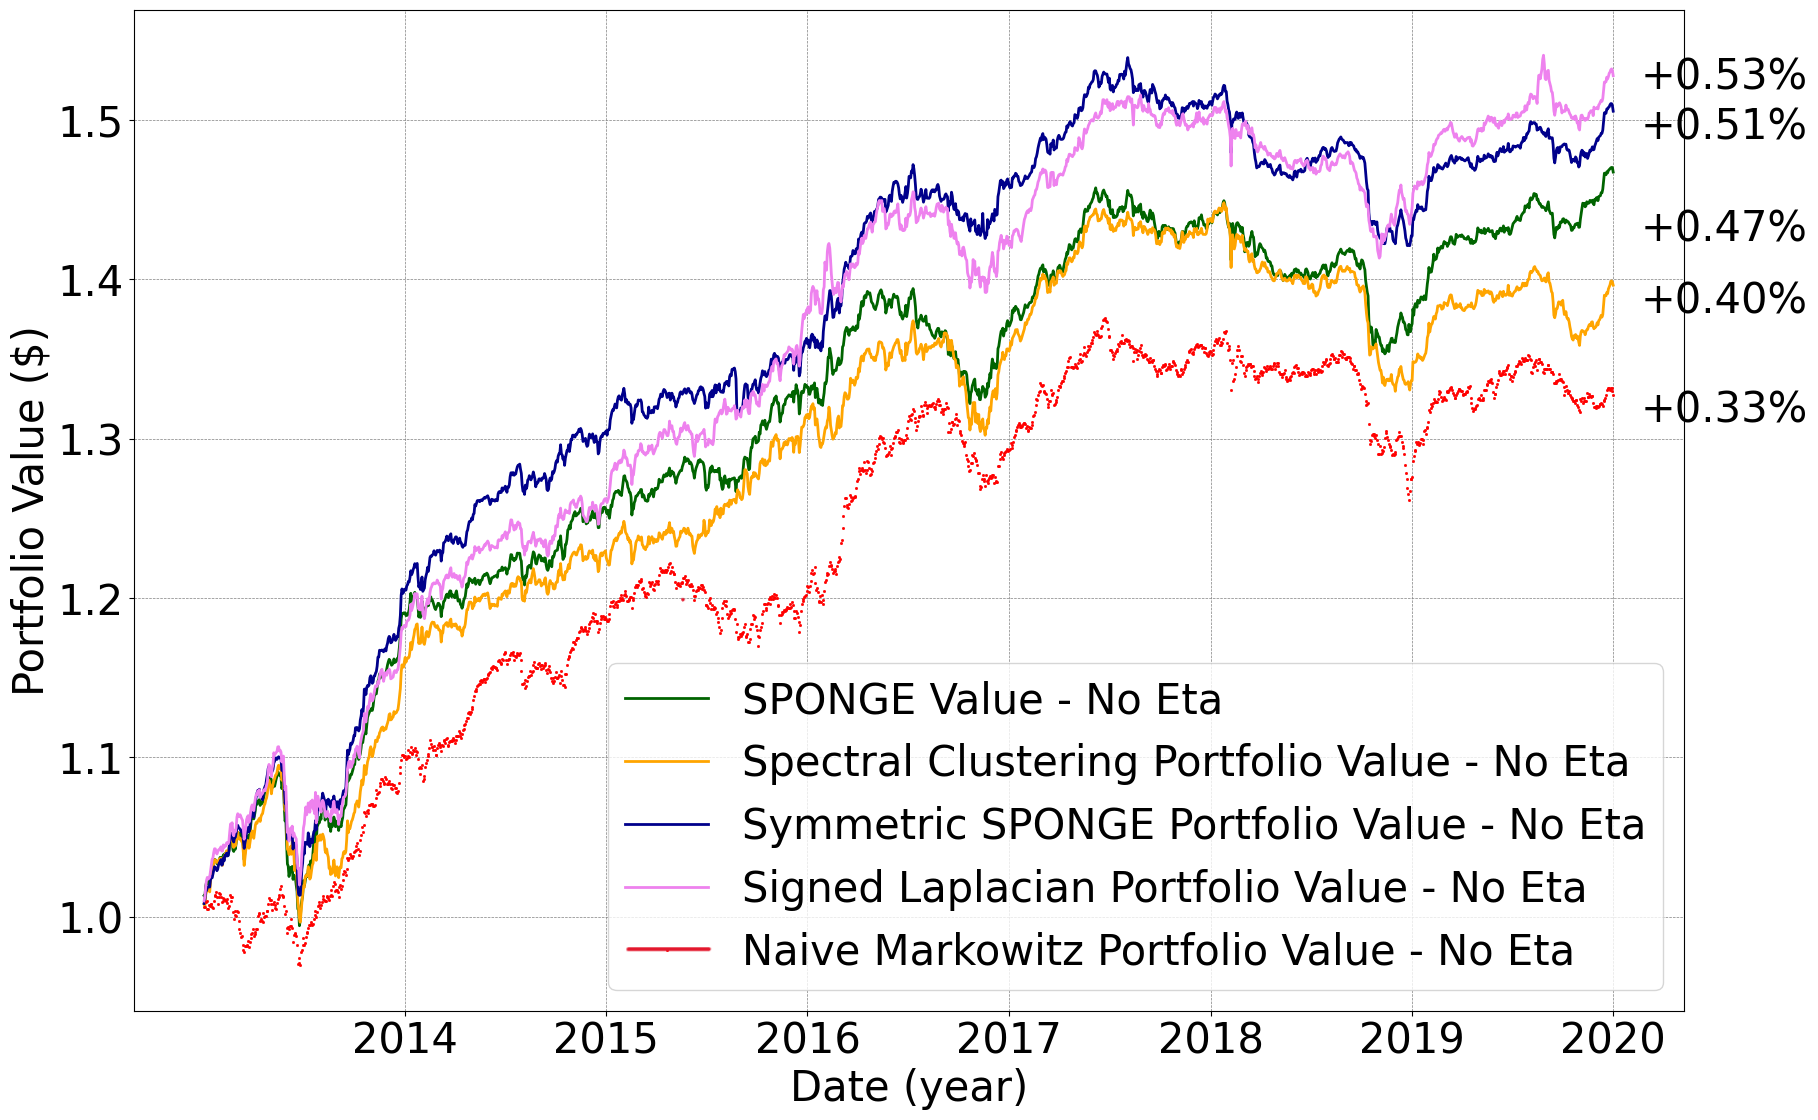
\includegraphics[width=1.0\linewidth]{Source/No_eta_comparison.png}
  \caption{$\eta = 0$}
  \label{no-eta}
\end{minipage}
\caption{Portfolio clustering statistics for varying $\eta$.}
\end{figure}

\begin{itemize}
	\item improved prediction accuracy leads to enhancements in both returns and volatility ($\eta = 1$ denotes a perfect prediction)

    \mypv 
    \item $\eta = 0$ results in poorer performance in terms of returns and volatility, although it still achieves a Sharpe Ratio above 1
    \mypv 
    \item \red{cluster-based strategies attain lower volatility and higher returns, compared to the naive Markowitz approach} 
\end{itemize}

\vfill 
\end{frame}
%%%%%%%%%%%%%%%%%%%%%%%%%%%%%%%%%%%%%
%%%%%%%%%%%%%%%%%%%%%%%



\begin{frame}{Performance statistics for $\eta=0$}
   \footnotesize
\vfill

% \textbf{\underline{No forecasting $\eta = 0$:}}

\begin{table}[H]
    \centering
     \renewcommand{\arraystretch}{0.99}
    \begin{tabular}{|c|c|c|c|c|c|}
    \hline
    Metric | Portfolio & Naïve & SPONGE  & SPONGE sym & SL & SC \\ \hline
    Return & \textcolor{red}{32.76\%} & 46.72\% & 50.53\% & \textcolor{blue}{52.77\%} & 39.62\%\\ \hline
    Annualized Return & \textcolor{red}{4.14\%} & 5.64\% & 6.03\% & \textcolor{blue}{6.26\%} & 4.89\% \\ \hline
    Daily Volatility & 0.24\% & \textcolor{blue}{0.23\%} & \textcolor{blue}{0.23\%} & \textcolor{red}{0.25\%} & 0.24\% \\ \hline
    Annualized Volatility & 3.82\% & 3.69\% & \textcolor{blue}{3.58\%} & \textcolor{red}{3.93\%} &3.86\%\\ \hline
    Sharpe Ratio & \textcolor{red}{1.08} & 1.52 & \textcolor{blue}{1.68} & 1.59 &1.27\\ \hline
    Sortino Ratio & \textcolor{red}{1.48} & 2.01 & \textcolor{blue}{2.14} & \textcolor{blue}{2.14} & 1.63\\ \hline
    \end{tabular}
    \vspace{3mm}
\caption{Performance metrics - $\eta = 0$. SL: Signed Laplacian; SC: plain spectral clustering on the absolute value correlation matrix. \blue{Blue}/\red{red} denote the \blue{best}/\red{worst} performance for each metric.}
\label{tab:perf metrics eta=0}
\end{table}

%\begin{figure}[H]
%\centering
%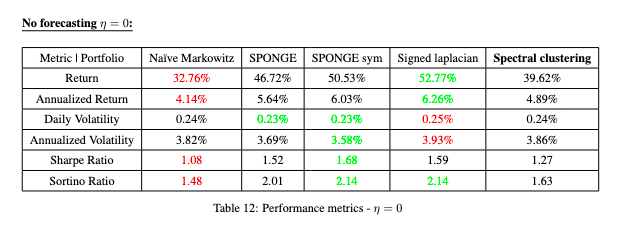
\includegraphics[width=0.1\linewidth, trim={0 1.3cm 0 0},clip]{Source/eta0_hc.png}
%\caption{Portfolio clustering statistics for $\eta=0$.} 
%\end{figure}

\vfill 

\begin{itemize}
\item Naive Markowitz typically attains  the worst performance metrics
\item Signed clustering methods attain the best performance compared to plain spectral clustering (SC)
\end{itemize}

\vfill 
\end{frame}




%%%%%%%%%%%%%%%%%%%%%%%%%%%%%%%%%%%%%%%%%%%%%%%%%%%%%%%%%%%%
\section[Conclusion]{Conclusion and future work}

\begin{frame}{Conclusions}
   
\vfill
% In this work, we introduced an alternative framework for portfolio construction that leverages graph clustering algorithms to address the complexities of Markowitz Mean-Variance Optimization in large asset universes. To test this method, we built a backtesting framework that revealed compelling results. In terms of Sharpe ratio, the portfolio strategies are ranked, starting from the best one, as follows: Markowitz clustering with EWA, Markowitz with clustering but without EWA, naïve Markowitz portfolio, SP 500 Index and equally weighted portfolio. Using the symmetric SPONGE clustering algorithm, this combination achieves a Sharpe ratio of $3.52$ and a Sortino ratio of $4.99$. These performances demonstrate that while Markowitz optimization is effective in reducing portfolio volatility, it becomes more efficient when coupled with a clustering method to reduce dimensionality, and a better estimation of the covariance to address non-stationary issues inherent in the time series of returns. Under market stress, our portfolio strategy continues to perform well, such as in 2018 when the SP 500 lost more than $40$\% of its value, and our portfolio strategy still showed positive returns. Another interesting finding is that the cluster-driven portfolios perform best with $K=24$ clusters, which could be aligned with its economic interpretation, as there are $24$ industry groups within GICS®, and the fact that the dimensionality remains quite high, preserving more effectively the information content. 

\begin{itemize}
    \item  backtesting framework ranks portfolio strategies by Sharpe Ratio as follows:
        \begin{itemize}
            \item Markowitz clustering with Exponential Weighted Average (EWA)
            \item Markowitz clustering without EWA
            \item naïve Markowitz portfolio
            \item S\&P500 Index
            \item equally weighted portfolio
        \end{itemize}
        
\mypv
    \item highest Sharpe and Sortino Ratios are achieved with signed clustering methods 
    % symmetric SPONGE clustering
    % Sharpe ratio of 3.52 and a Sortino ratio of 4.99 are achieved with symmetric SPONGE clustering.
    % QQQ
    
    \item under market stress, the portfolio strategy remained resilient, showing positive returns in 2018 despite the S\&P 500's 40\% decline.
    
    \item optimal results were attained for \(K = 24\) clusters, aligning with the 24 GICS® industry groups and preserving high information content.
\end{itemize}





\vfill 
\end{frame}
%%%%%%%%%%%%%%%%%%%%%%%%%%%%%%%%%%%%%%%%%%%%%%%%%%%%%%%%%%%%




%%%%%%%%%%%%%%%%%%%%%%%%%%%%%%%%%%%%%%%%%%%%%%%%%%%%%%%%%%%%
\begin{frame}{\large Future work}
   
\vfill 

% While our research centers on comparing the performance of our clustering and forecasting-based strategy against traditional Markowitz optimization, our framework is highly versatile and can be tailored with various parameters, including different target returns, alternative optimization methods, and diverse constituent weights. Future exploration of these configurations could further improve the effectiveness of the strategy under varying market conditions. 

% Looking ahead, several avenues for improvement are worth considering. For the graph construction component, exploring alternative correlation metrics could lead to different covariance matrix estimates. Additionally, examining various clustering methods might provide further insights, as our results indicate that clustering efficiency varies across different scenarios. Incorporating Markowitz optimization within clusters for determining internal weights could integrate our approach with those suggested by \cite{León}, \cite{Tola} and \cite{Gatta}, potentially further enhancing performance. Moreover, leveraging advanced covariance forecasting techniques (see \cite{zhang2022graphCov,gnn2023graphCov}, and also  \cite{CaoZheng} for a method and a review), and enhancing EWA with cross-validation approaches (see \cite{TanZohren}), GARCH models, or deep learning methods, could offer further improvements to our proposed trading strategy. 

Our framework focused on comparing clustering and forecasting-based strategies with traditional Markowitz optimization; is flexible and can be customized with:
        \begin{itemize}
            \item different target returns
            \item alternative optimization methods 
            \item varied constituent weights
            % QQQ
        \end{itemize}

\mypv
Looking ahead, several avenues for improvement are worth exploring:
\begin{itemize}
	\item alternative correlation metrics for graph construction
    \mypv 
    \item  alternative clustering methods
    \mypv 
	\item integration of factor models 
	\mypv 
	\item apply Markowitz optimization within clusters to enhance weight allocation 
    % , as suggested by related research 
    (\cite{León, Tola, Gatta}) 
	\mypv  
	\item leverage advanced covariance forecasting techniques % (\cite{zhang2022graphCov, gnn2023graphCov, CaoZheng}) 
    to improve the trading strategy

     \item enhancements to EWA through cross-validation, GARCH models, or deep learning methods (\cite{TanZohren})
\end{itemize}

\vfill 
\end{frame}
%%%%%%%%%%%%%%%%%%%%%%%%%%%%%%%%%%%%%%%%%%%%%%%%%%%%%%%%%%%%





% \section[MRA]{SSSS}

% \begin{frame}
%     For cyclically shifted signals we estimate lags with circular CCF.
    
%     For time series variables $X_t$ and $Y_t$ of length $T$, 
%     \begin{equation}
%         \widehat{Corr_C(X_t,Y_t)}[n]  = \frac{\sum_{t=0}^{T-1}X[(t+n)\mod T] \cdot Y[t]}{|X||Y|},\text{  }n=0,\dots, T-1.
%     \end{equation}
%     Similarly, the lag is defined as \footnote{We ignore the negatively correlated lead-lag structure.}
%     \begin{equation}
%         \mathcal{L}(X_t,Y_t)=\min \argmax_{0\leq n\leq T-1} Corr_C(X_t,Y_t)[n],
%     \end{equation}

% \end{frame}
 

  

% \begin{frame}{Future Work}
%     \begin{itemize}
%         \item Multi-factor mixed-membership analysis: model each asset as reacting to multiple factors, each one with its own lag and exposure.
%         \item Confidence weighted portfolio: Derive a confidence measure or uncertainty bound for the lag estimates, and apply the results to optimize trading portfolio weights.
%     \end{itemize}
% \end{frame}


 

\begin{frame}[noframenumbering]
\centering
\Large
Thank you!

\vspace{.5cm}
\Large
Q \& A
\end{frame}

\begin{frame}[allowframebreaks,noframenumbering]{References}
    \printbibliography
\end{frame}

% \section{Appendix}

\end{document}









